%!TEX program = xelatex
\documentclass[a4paper]{ctexart}
\setCJKfamilyfont{fzsongti}{FZShuSong-Z01S}% 定义方正书宋
\newcommand{\fzsongti}{\CJKfamily{fzsongti}}
\usepackage{listings} 
\usepackage{geometry}
\usepackage{booktabs}
\usepackage{graphicx}
\usepackage{tabularx}
\usepackage{multirow}
\usepackage{enumitem}
\usepackage[bottom]{footmisc}
\renewcommand{\multirowsetup}{\centering}

\geometry{
    left=23mm,
    right=23mm,
    top=23mm,
    bottom=23mm,
}

\setlength{\parskip}{0.5em}

\title{\Huge PetLover 商业模式设计文档}

\author{
  项目成员:\\
  姬筠刚 191250055(PM)\\
  陈梓俊 191250016\\
  丁炳智 191250024\\
  刘庭烽 191250093\\
}
\date{\today}

\begin{document}

\maketitle

\centerline{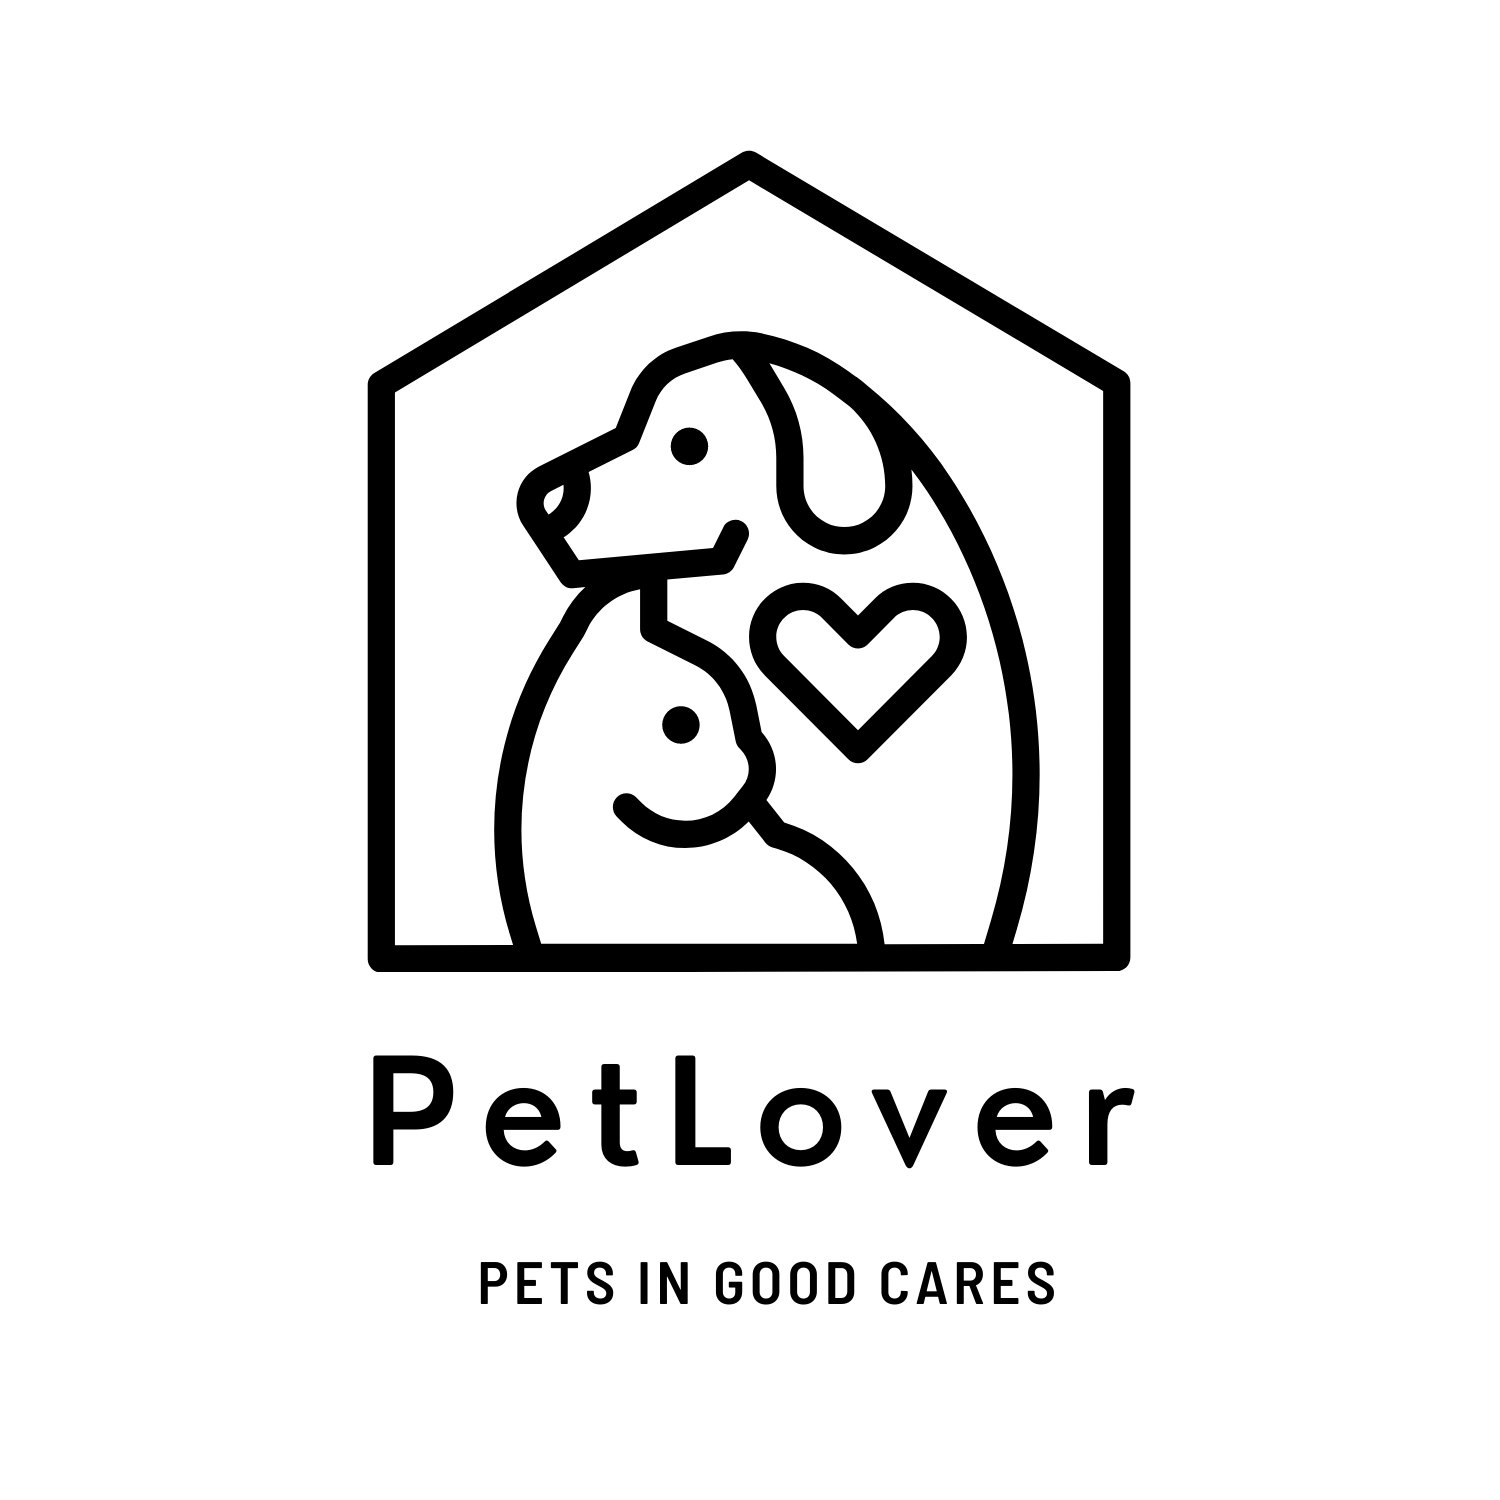
\includegraphics[]{logo.png}}

\newpage

\begin{abstract}
  本项目名为PetLover,是由本小组于2021年秋季学期《需求与商业模式创新》课程大作业中设计的软件产品项目。此文档为商业模式设计文档,主要内容包含本项目的商业模式设计有关的六大设计方法,包括客户洞察、构思、视觉化思考、模型构建、讲故事和场景。
\end{abstract}



\tableofcontents

\newpage

\setlength{\parskip}{1em}


\section{度量数值}

本文档共包含了:客户洞察部分4个客户群体的移情图;构思部分5个候选创意;模型构建更新的画布要点数量为39个(新增一个关键业务“上门服务”),关联关系19条,引用的调研报告和新闻报道为15篇;讲故事部分故事数量为5个(其中4个客户视角故事,1个公司视角故事);场景部分要点数量为7个(分别是场景IP、场景分发、了解并评估、购买并传递获得、交互、售后、评价与复购),涵盖4个客户群体(与讲故事部分一致)的场景补充。

\section{视频链接}

PetLover团队商业模式画布可视化故事讲述以及讨论花絮视频链接如下:

https://www.bilibili.com/video/BV1aR4y1t7Qw/

\section{商业模式设计}

\subsection{客户洞察}

\subsubsection{宠物爱好者}
\begin{enumerate}[label=\alph*.]
  \item 看:有很多对宠物情有独钟的客户,他们或自己拥有爱宠,或因为自身条件无法饲养宠物。他们往往会在各大新媒体平台浏览关于各类宠物的短视频或动态,满足心理上对萌宠的强烈需求,做到“云吸宠”,也会同身边的人(如邻居、朋友等)交流宠物饲养的经验、碎碎念等等,在爱宠需要食物、洗刷用品、药品时他们会在电商平台上购买相关物品,在爱宠得病或需要接种疫苗时他们又会到当地宠物医院咨询并寻求相关医疗服务。而这类用户为了满足这几项需求会遇到这样几个问题:需要跨多个平台寻求服务,效率较低;大多数社交平台宠物爱好者密度较小,没有形成爱宠社区,很难与其他用户产生共鸣;获取宠物饲养经验的途径较少。
  \item 听:朋友和邻居会将宠物饲养技巧或自己爱宠的萌点讲给他们听;新媒体博主的各种吐槽和爱宠日常行为分享;养宠费用高昂会打磨他们饲养宠物的兴趣;他们了解网络社区概念,宠物主题的网络社区可以集中具有共同兴趣的访问者,但让他们头疼的是大多宠物社区的信息不可信且充斥着广告信息。
  \item 想与感受:对于计划养宠的客户,他们希望能有一个线上平台能够全方位的了解各种宠物的特征信息并能更加划算、可靠的购买宠物;对于拥有宠物的客户,他们深受虚假信息、广告信息的困扰,希望向别人请教养宠技巧、快速获得优质信息,同时也希望分享自己爱宠的动态获得他人的肯定和情感上的共鸣,他们也思考如何才能低成本的饲养宠物、到哪里去买便宜且可靠的宠物用品、如何方便快捷的为爱宠寻求医疗服务;对于不养宠的客户,他们喜欢萌宠而希望做到云养宠。
  \item 说与做:吐槽养宠感受;分享养宠日常;购买宠物及其用品;咨询宠物医疗服务;通过现有社交平台结识宠物爱好者来分享或获得养宠经验。
  \item 痛点:跨平台寻求服务,不方便;虚假信息和网络信息过多,影响判断;身边养宠爱宠人士较少,很难同身边的人获得情感上的共鸣,分享宠物日常途径较少,分享得到的反馈较少;宠物用品昂贵且购买途径较少、质量难以得到保证;由于大多宠物医院都是线下服务,寻求宠物医疗服务需要耗费大量时间。
  \item 收益:相对较低价格的宠物及其用品,降低养宠成本;使用集社区论坛、医疗服务、宠物及其用品购买、物流服务、售后服务、质量保障于一体的平台,分享能得到反馈,购买质量得到保证,养宠更加便利;线上医疗咨询,上门医疗服务,减少爱宠求医浪费的时间。
  \item 宠物爱好者移情图如下:
\end{enumerate}
\begin{center}
  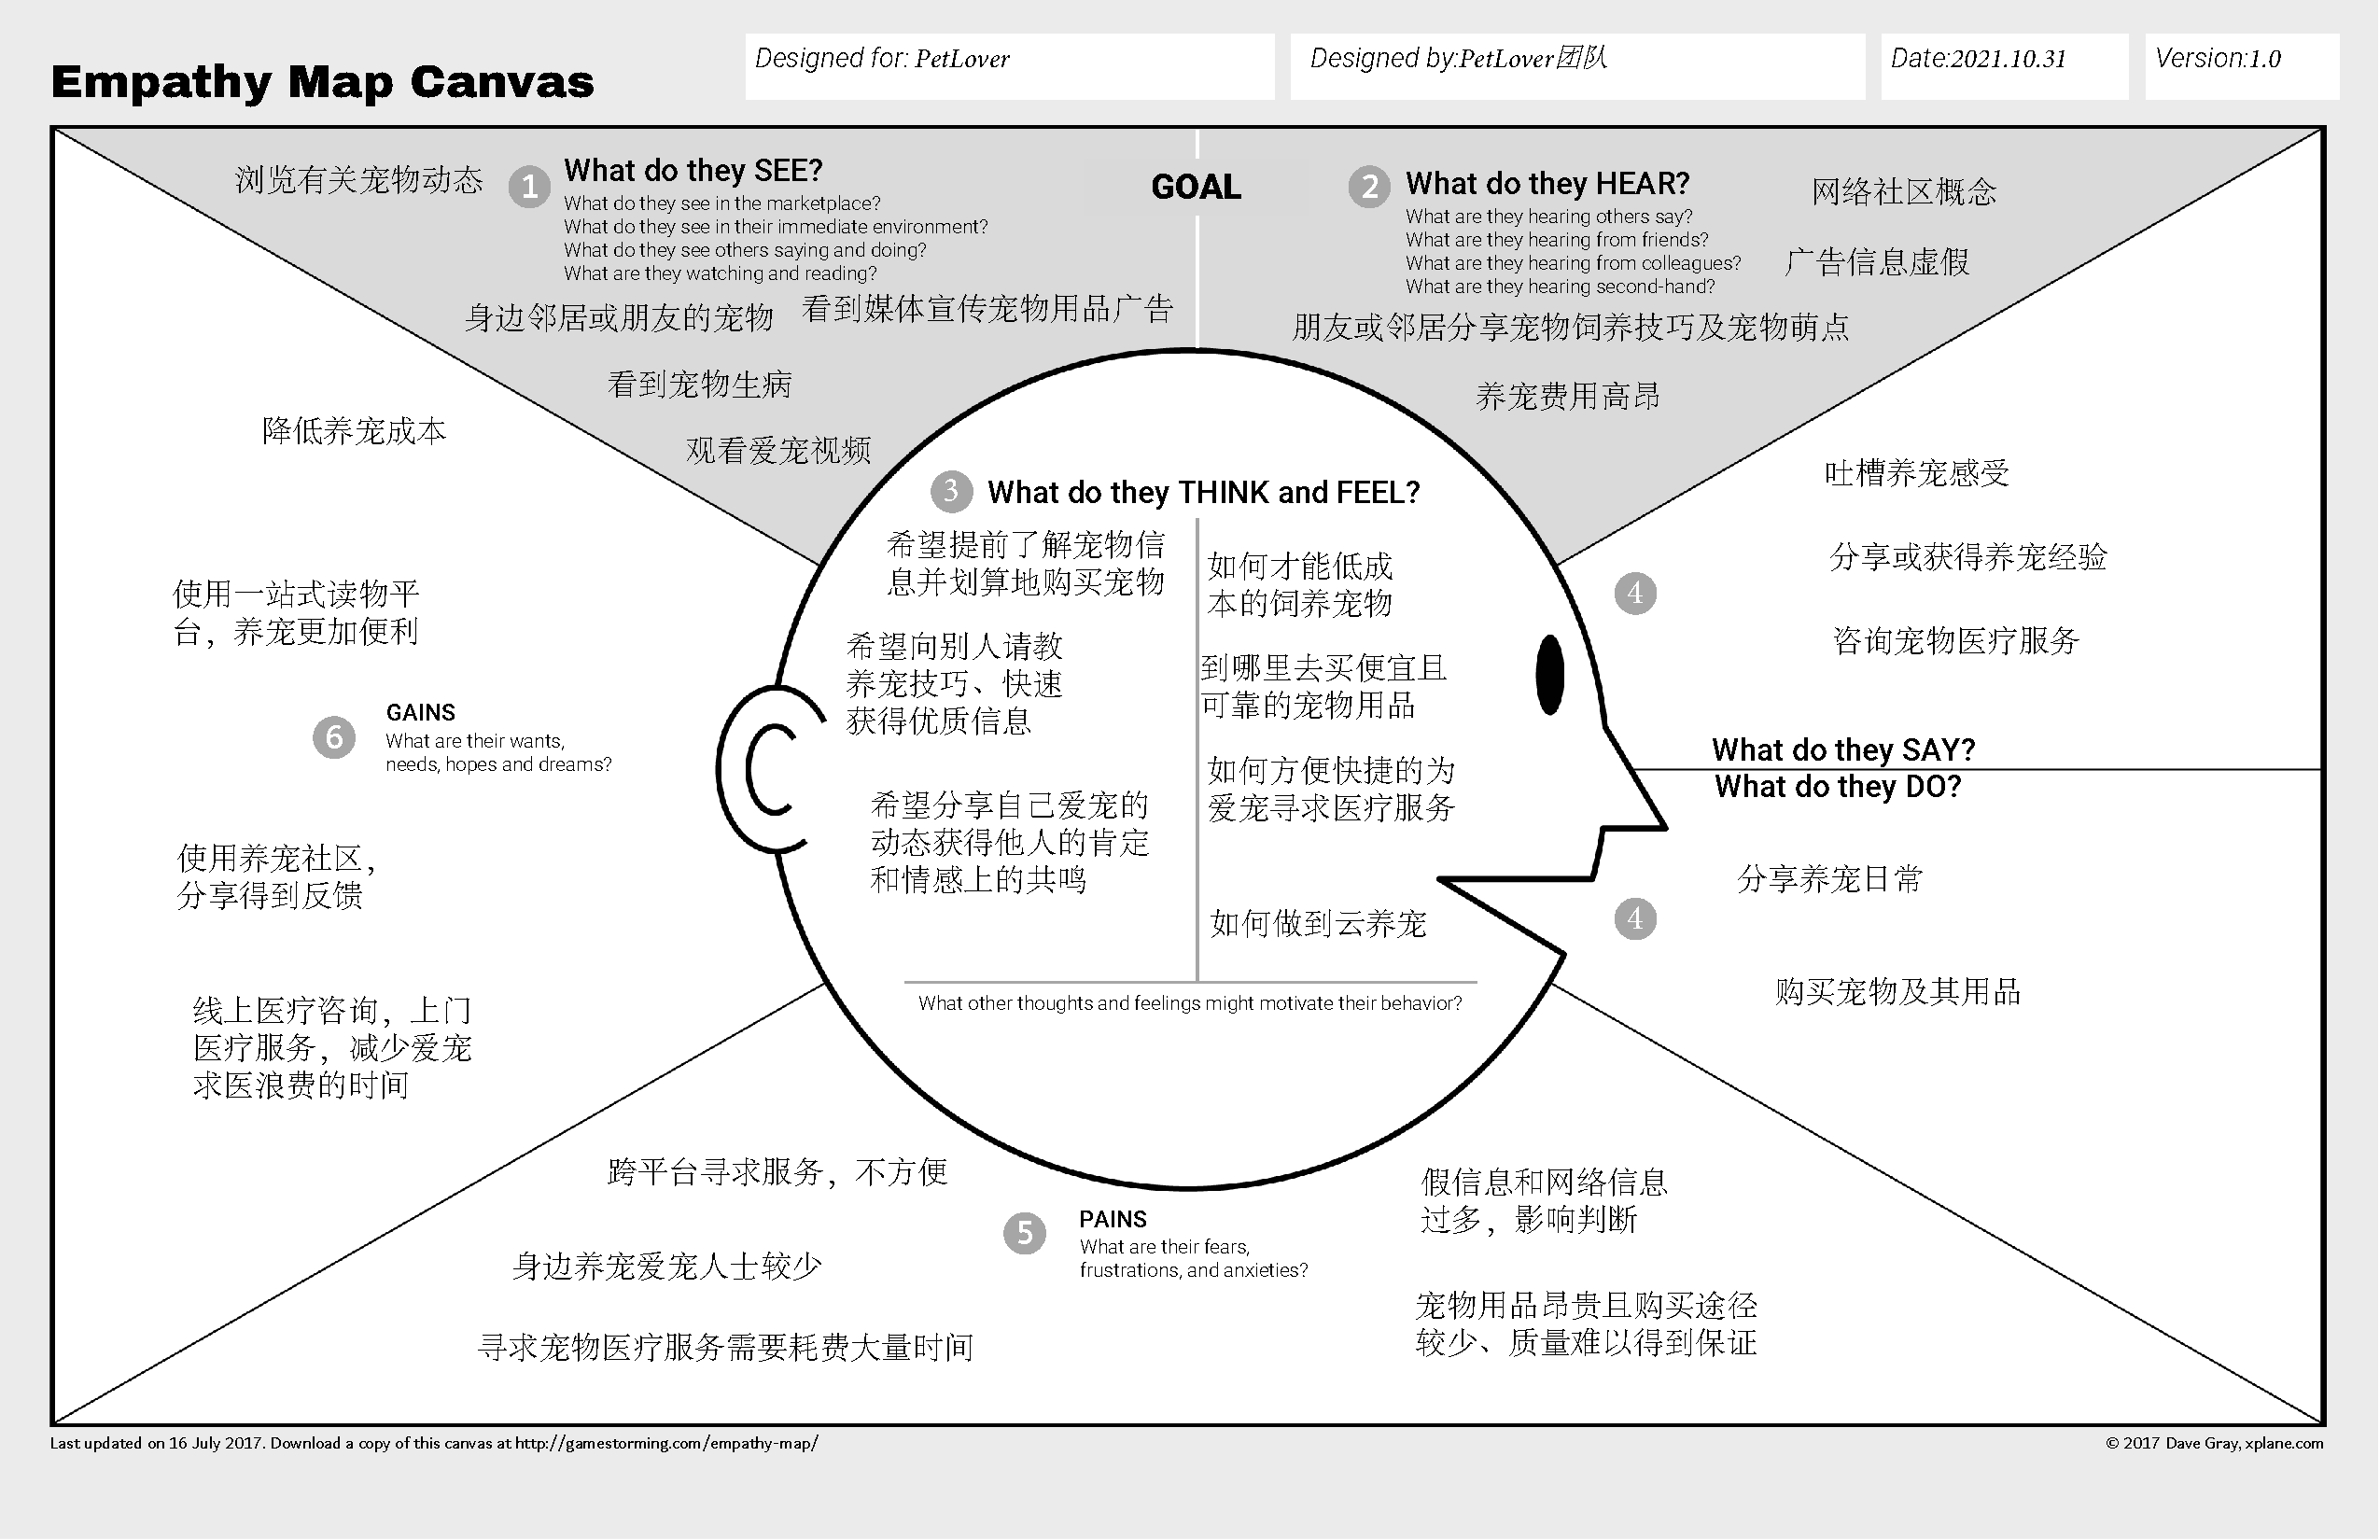
\includegraphics[width=16cm]{./移情图/宠物爱好者}
\end{center}

\subsubsection{宠物医疗行业从事者}
\begin{enumerate}[label=\alph*.]
  \item 看:这类用户有专职也有兼职。在线下环境中,专职宠物医疗从事者大多通过在宠物医疗机构工作,周围是同事、宠物患者及其主人,他们习惯于同宠物主人打交道并跟他们沟通宠物身体状况,为宠物提供人道主义的医救方式,和同事交流宠物治疗经验。而很多地区宠物医疗机构覆盖率低,具体见“听”部分,宠物医疗从事者会错过很多未覆盖地区的宠物医疗服务,收入较低,兼职者参与宠物医疗工作不方便。
  \item 听:中国宠物医疗行业整体运行处于低水平状态,宠物医生人才储备不足,宠物医疗行业从事者就业机会比较多,但另一方面,宠物医院等医宠物疗机构大多分布在一二线城市,分布密度城市中心>社区>街道,对小城市的宠物医疗行业从事者不利;互联网+迅速发展,宠物医疗行业商业模式正在向互联网+靠拢;目前线上医疗咨询成为一个趋势。
  \item 想与感受:他们希望能够增加服务机会,提高收入;希望能在线上提供医疗咨询获得收入,兼职宠物医疗从事者希望有一种线上接单的方式来增加兼职工作的便利性,以此实现自身宠物医疗能力的价值并获取收益;宠物医院经营者希望增加客流量,扩大经营规模。
  \item 说与做:与宠物主人互相吐槽养宠的麻烦以及交流如何才能减少养宠麻烦,为宠物主人提供医疗服务便利,实现共赢;提供线上咨询服务;通过互联网、电话、邮件等媒介提供宠物医疗上门服务。
  \item 痛点:经营规模小,服务地域范围小,收入较少;兼职宠物医疗从事者在现有网络及现实环境下工作机会少。
  \item 收益:利用互联网平台扩展业务范围,提供线上宠物医疗咨询服务,扩大潜在服务区域,使得服务不受地域限制,做到上门医疗服务;获得更多订单,赚取更多收入;兼职者能够随时随地利用互联网平台参与宠物医疗服务。
  \item 宠物医疗行业从事者移情图如下:
\end{enumerate}
\begin{center}
  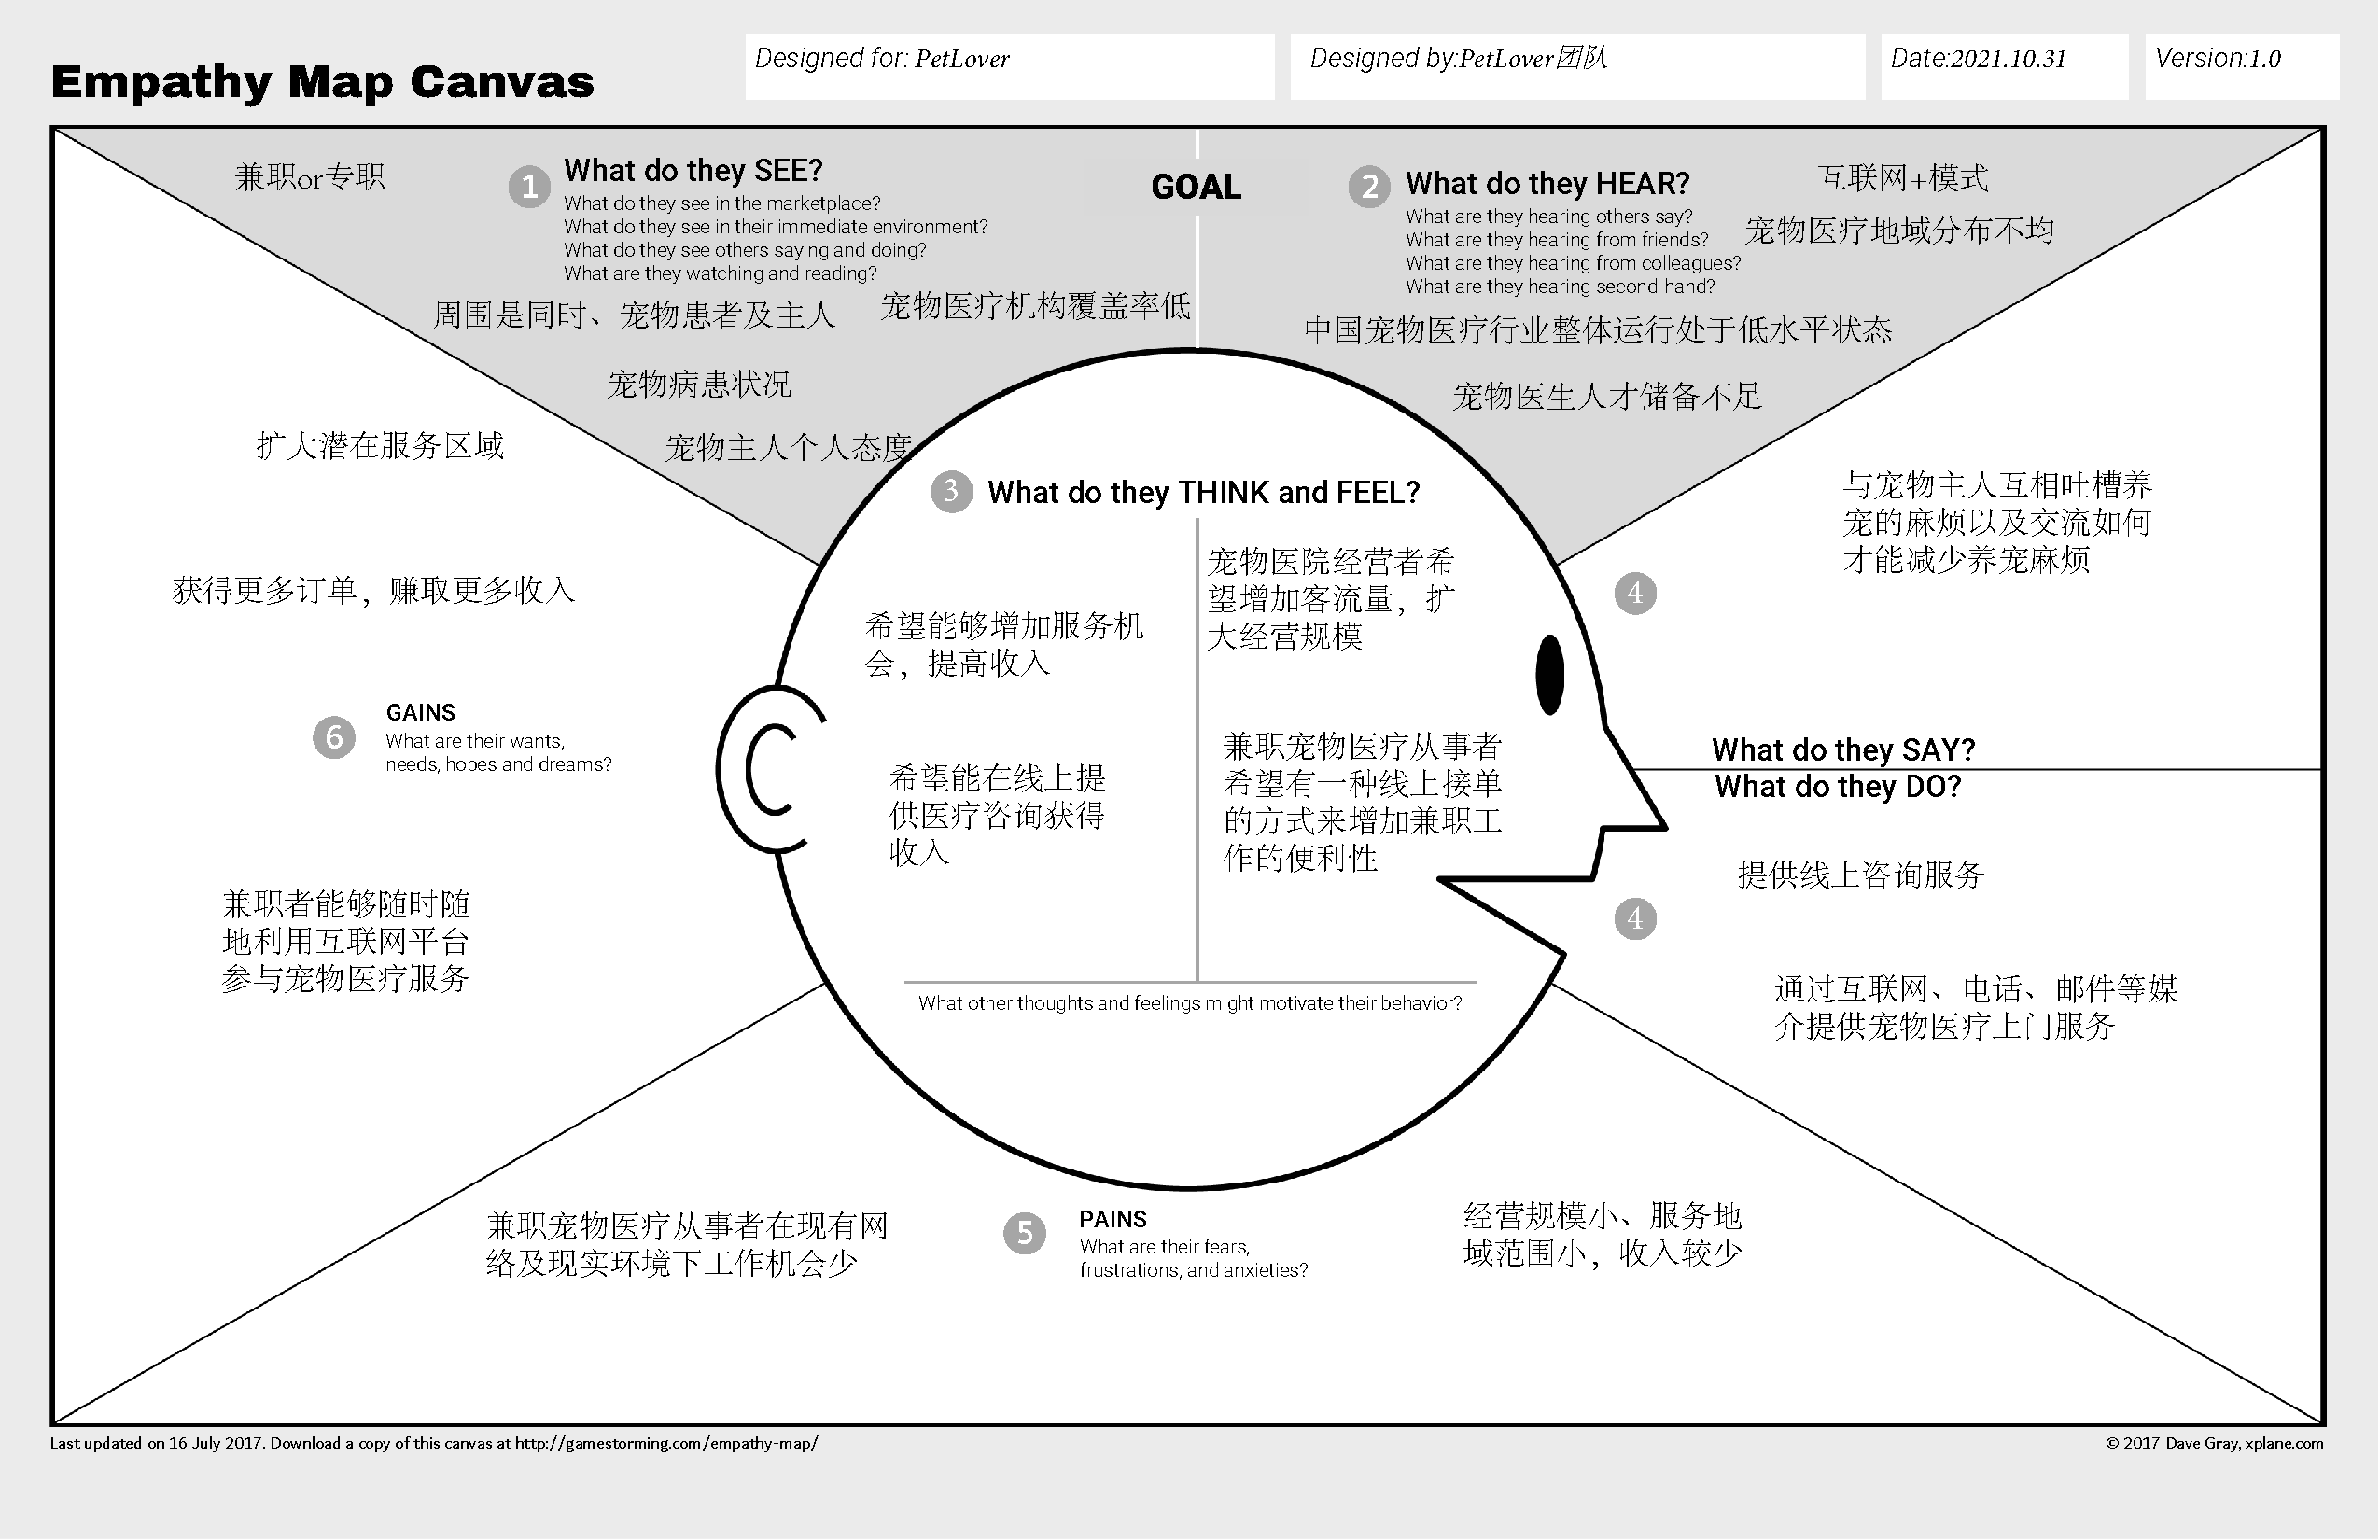
\includegraphics[width=16cm]{./移情图/宠物医疗行业从事者}
\end{center}

\subsubsection{宠物及用品供应商}
\begin{enumerate}[label=\alph*.]
  \item 看:宠物及用品售卖途径多元化;他们身边有很多相关产品竞争者;常常接触类似视短视频、长视频、微博等新媒体的博主,让他们进行宠物及产品品牌的宣传;通过电商平台售卖。
  \item 听:电商平台快速发展,冲击了实体商店的售卖;竞争者争相进军电商平台,抢占电子市场;新媒体成为广告投放的主流,宠物及用品供应商投放更多广告以提升销量;物流服务行业发展迅速,该类用户与物流服务行业合作密切。
  \item 想与感受:希望能针对特定人群投放广告,降低广告成本的同时也能提高销量;希望能有一个平台证明他们产品的可靠性以及广告信息的真实性,以增加买家对他们的信任,且打击假冒伪劣产品,公平竞争;希望降低房租等成本,降低产品价格,提高销量,赚取更多收益。
  \item 说与做:通过正当渠道获取产品合格证明,并得到平台认可证书;与互联网结合,成为电商;与物流服务业进行合作;降低网购产品价格。
  \item 痛点:市场上有假冒伪劣产品侵占市场;存在大品牌的不公平竞争;在淘宝、京东等多元化电商平台不能做到面向特定受众,买家分流严重;也正是因为没有面向特定受众,广告投放规模要大,成本高。
  \item 收益:低成本,低价格,高销量,赚取更多收益;公平竞争。
  \item 宠物及用品供应商移情图如下:
\end{enumerate}
\begin{center}
  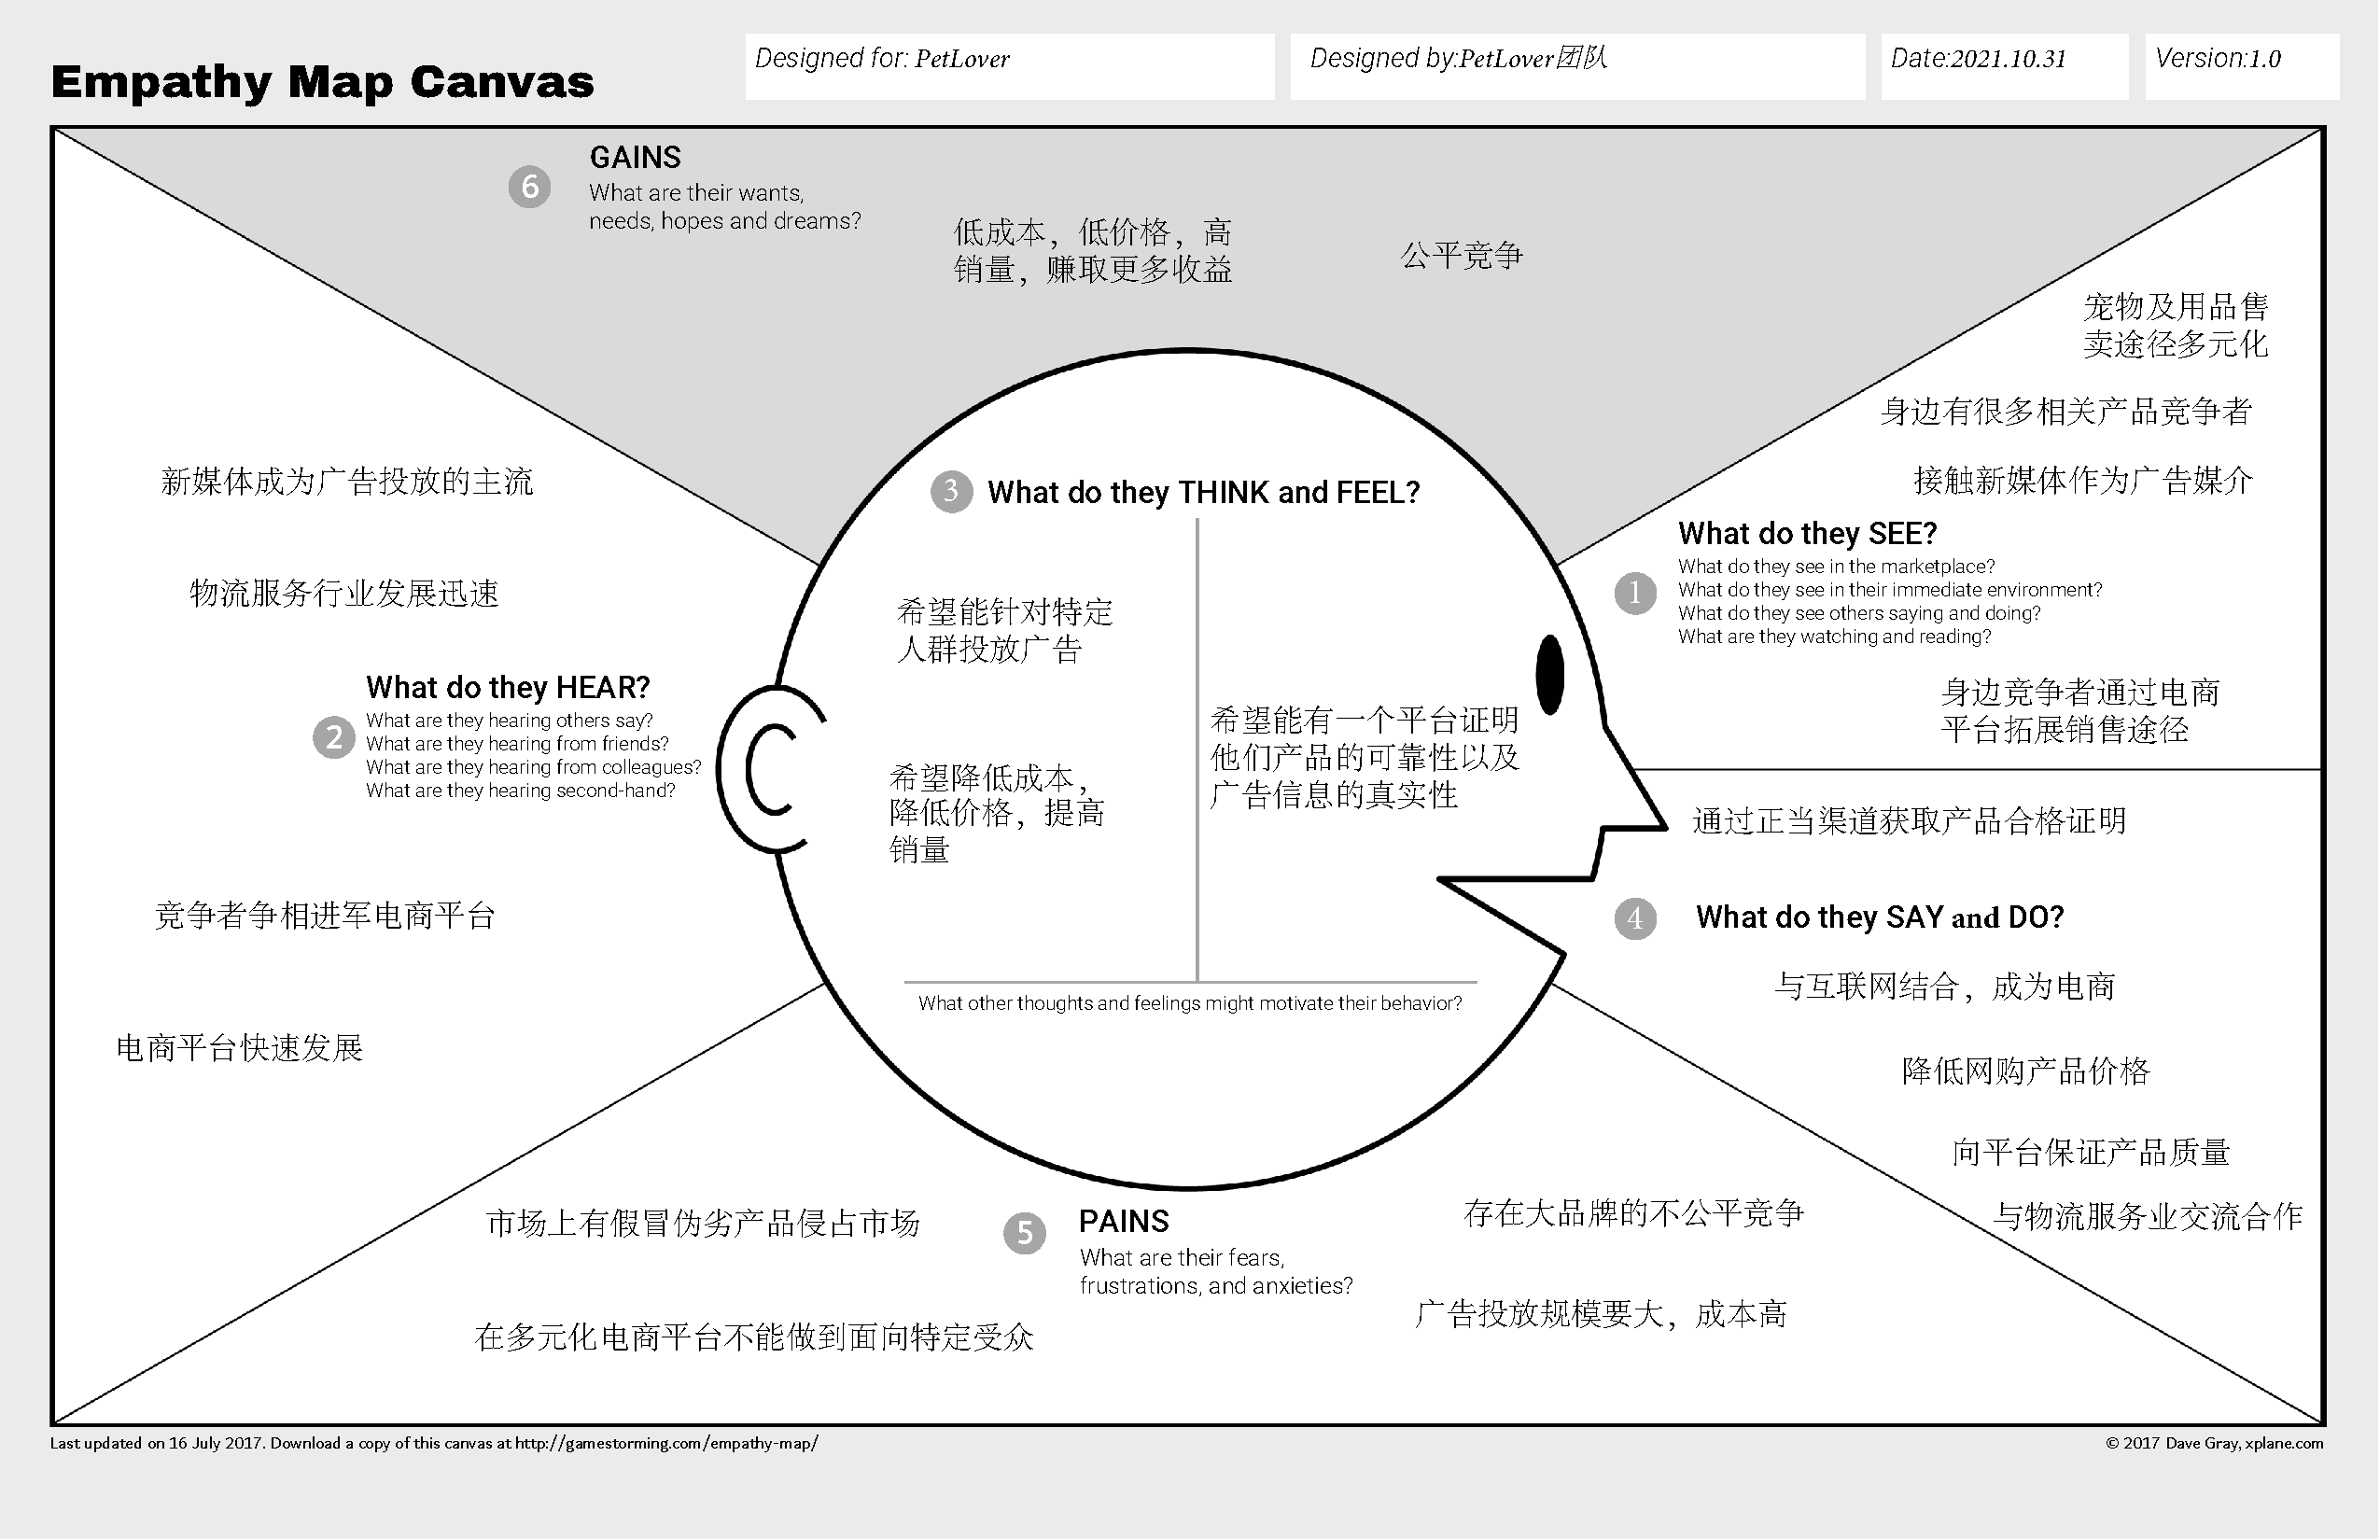
\includegraphics[width=16cm]{./移情图/宠物及用品供应商}
\end{center}

\subsubsection{动物保护志愿者}
\begin{enumerate}[label=\alph*.]
  \item 看:动物保护志愿者挤出零散时间投入动物保护这项事业中去,他们身边往往是志同道合、愿为动物保护付出的朋友;他们需要通过吸取新媒体工作者的经验来不断调整思想宣传的方式,留意身边人们对待动物的态度,矫正一些人们对待动物的行为,科普动物的爱好、习性等。
  \item 听:虐待动物、虐待宠物现象仍然存在,例如在高校经常有虐待校园猫的行为;当前周围人们的动物保护意识薄弱;中国小动物保护协会成立并得到进一步发展。
  \item 想与感受:希望人们加强动物保护意识;希望能有专门的新媒体平台供他们提供思想宣传活动,以传播爱护动物的人道主义思想;思考以何种方式能够高效率推进动物保护、思想传播这两项工作的进行,如何能够扩大志愿者组织影响力、招收更多志同道合的朋友投入这项事业中。
  \item 说与做:向人们宣传珍爱生命、倡导精神文明和发扬人道主义精神的思想;开展讲座、宣传平台来进行思想宣传、动物行为及爱好的科普;建立救护收容小动物的基地——爱心教育基地;救护动物;开设热线。
  \item 痛点:中国小动物保护协会关注度小,很少出现在大众视野中;动物保护志愿者大多是自愿且能力有限;地域广阔,无法做到动物救助和收容、思想宣传及科普工作的大范围覆盖。
  \item 收益:他们保护动物、维护动物的生存权利和不受虐待的权利的理想是崇高而现实的,作为动物保护志愿者完成他们的使命可以收获心灵上的慰藉;可以让动物保护思想深入大众的内心;相关志愿组织可以走入公众视野,扩大影响力并进一步引领大众保护动物。
  \item 动物保护志愿者移情图如下:
\end{enumerate}
\begin{center}
  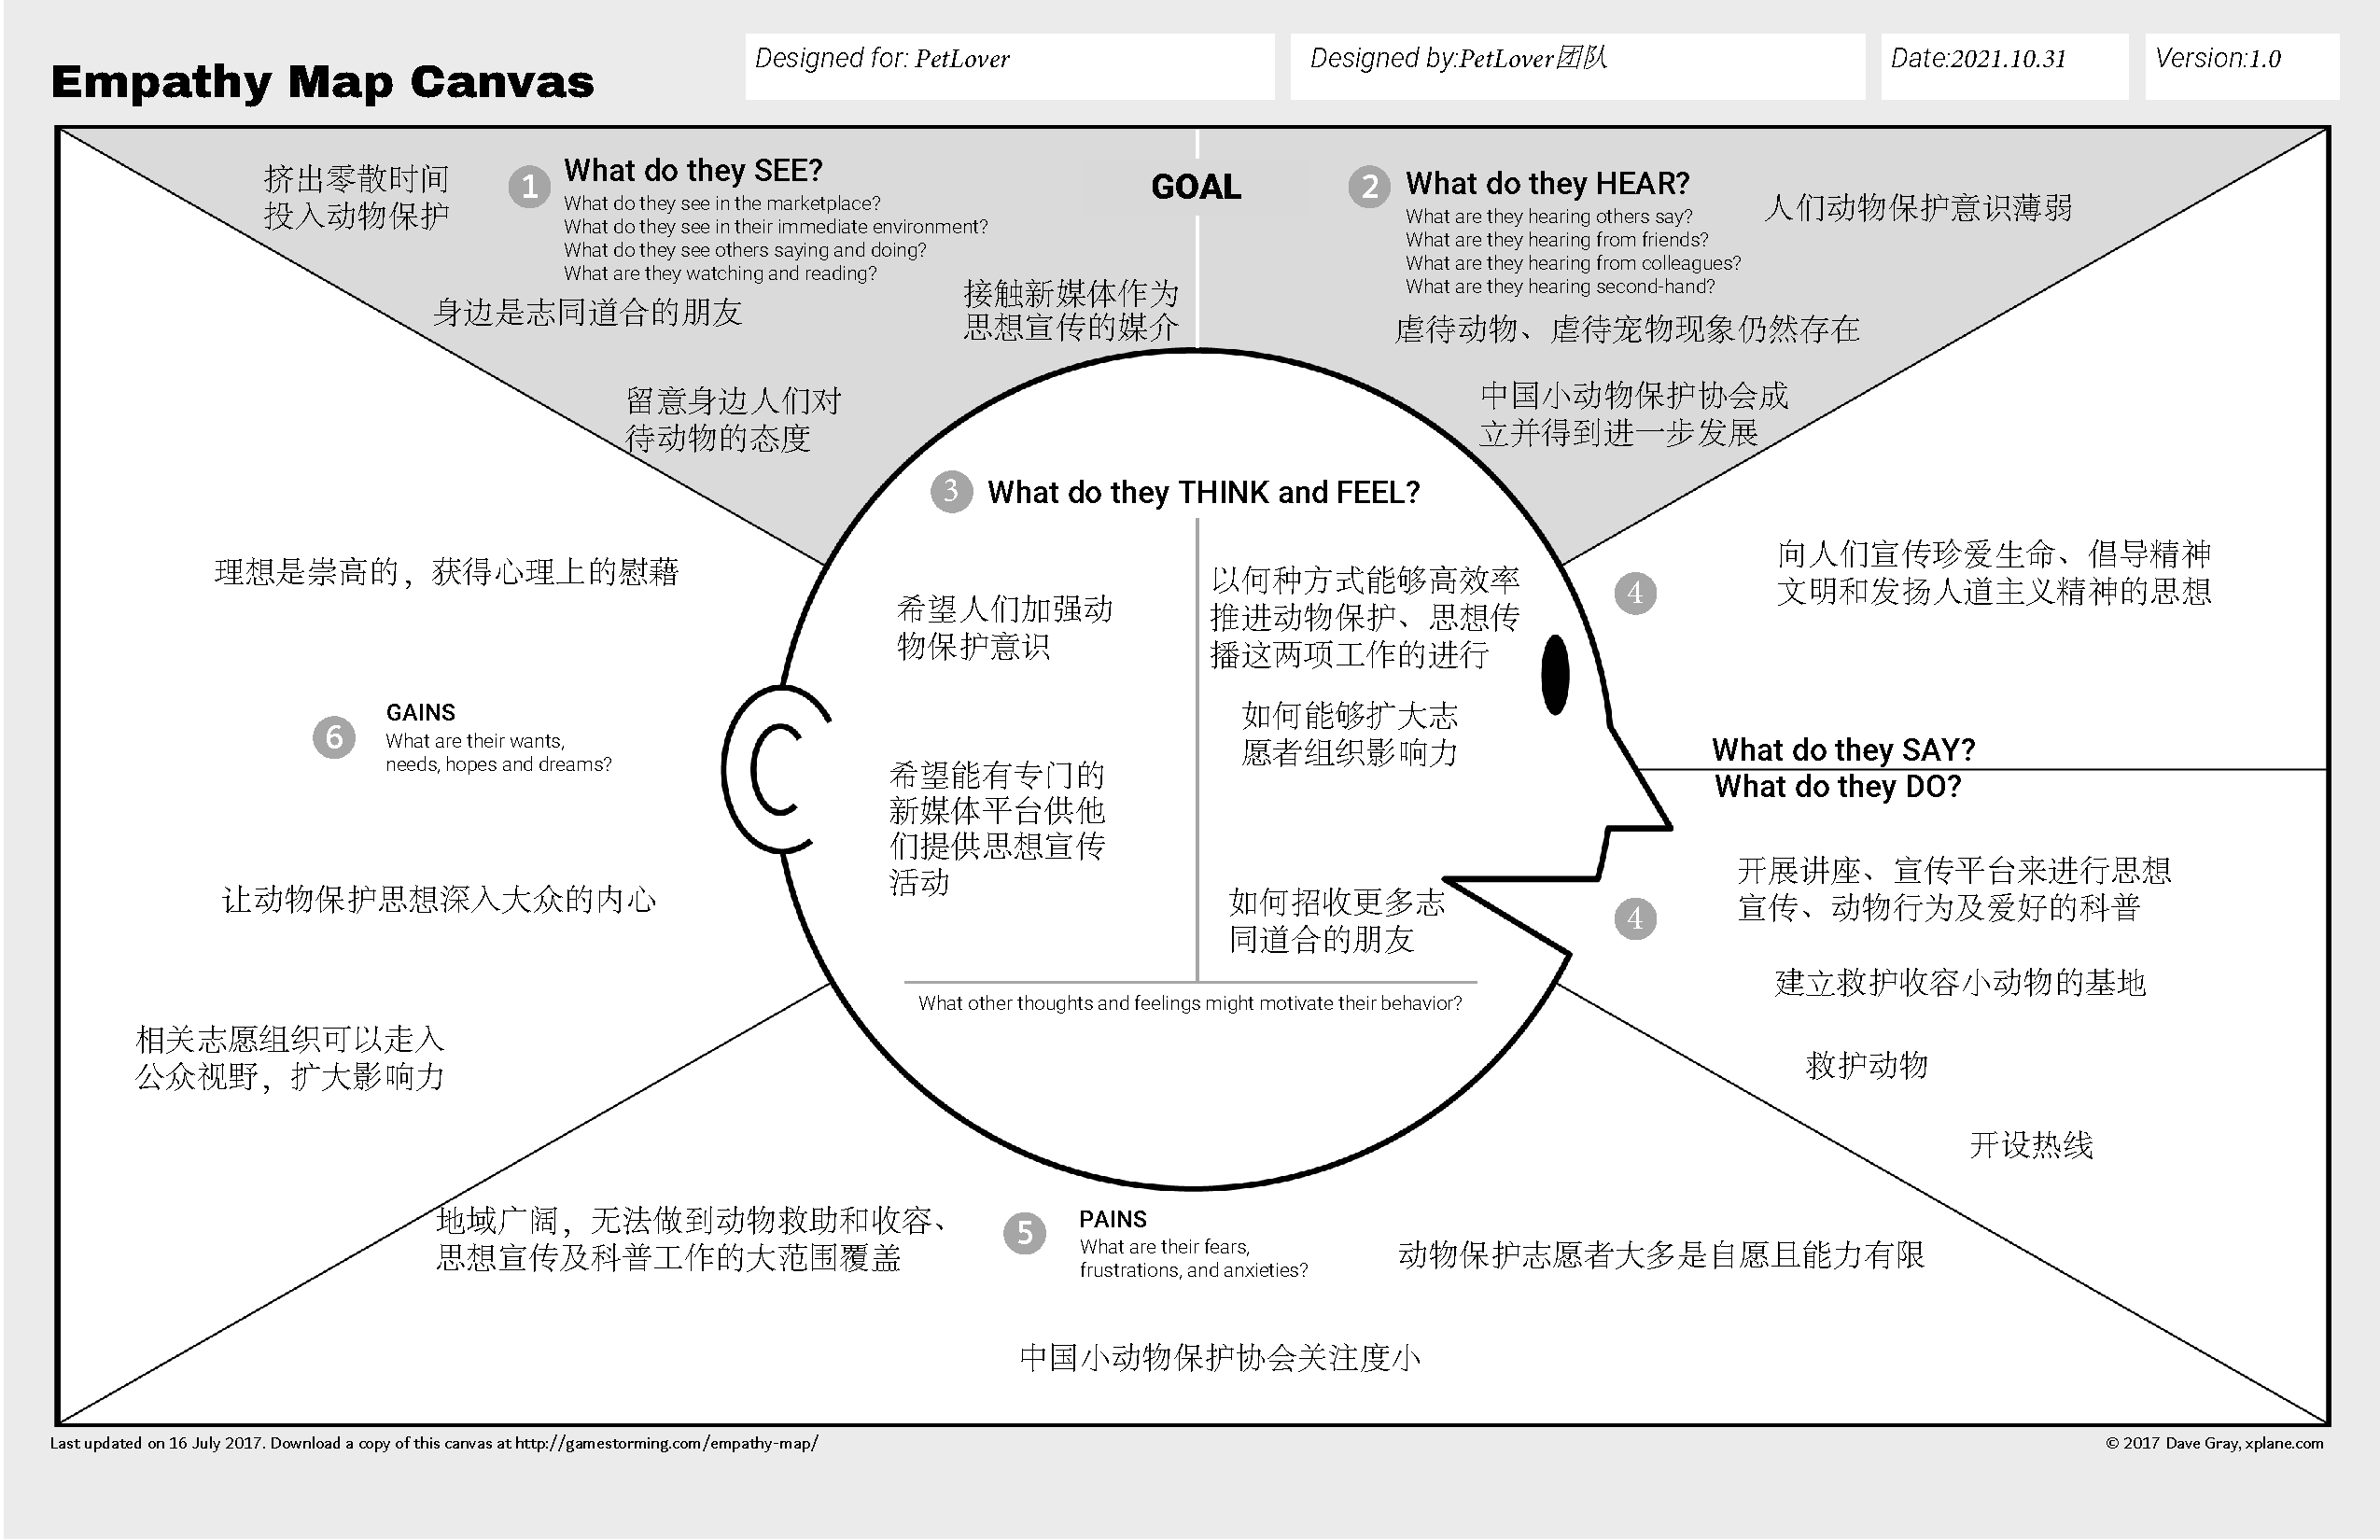
\includegraphics[width=16cm]{./移情图/动物保护志愿者}
\end{center}

\subsection{构思}

\subsubsection{基本商业构思}

基于上述客户洞察及相关分析,我们有理由认为:需要搭建一个以宠物购买为起点,持续提供宠物用品推荐/销售、宠物饲养日常分享社区、宠物疾病咨询等服务的一站式宠物交流平台,宣传并贯彻动物保护理念,提供宠物领养服务。通过提供上述多种服务,切实满足各类客户的需求,解决相关痛点,体现产品初心和价值。

\subsubsection{候选商业模式创意}
\begin{enumerate}[label=\alph*.]
  \item 资源驱动型——合作关系拓展,保证平台正常运转 
  \paragraph{驱动因素:}平台通过与线下宠物店/宠物医院进行合作,邀请“大咖”进行经验交流、好物推荐等方式,在“引进来”的同时实现“打出去”的目标,让一站式宠物买卖、交流服务从封闭社区扩展到面向更广大的客户群体。
  \paragraph{如果在平台建设初期,第三方合作者的数量不够怎么办?}1、平台建设初期,其商业模式和价值主张并不为人熟知,前期需投入一定成本进行平台宣传、大咖引进,展示平台的发展潜力,吸引第三方合作者主动加入。2、平台在持有一定数量的资源后,需要进行资源夯实和扩展,与优质的合作商建立长期合作伙伴关系,向用户提供优质资源的同时,也会让平台的影响力逐渐扩大,吸引更多优质资源。
  \paragraph{对整个商业模式画布的影响:}1、会对核心资源造成一定影响,使得其中实物资源得到相应扩充;2、重要合作关系会逐渐增多;3、在合作关系稳定后,对渠道通路中的大咖分享和专属服务会有扩展、未来收入会得到相应提升。
  \item 客户驱动型——基于用户建设宠物社区、活跃宠物交易 
  \paragraph{驱动因素:}用户的支持是驱动平台持续发展的巨大动力。爱宠社区是平台重要的价值传达媒介,其活跃度很大程度上由用户控制和决定;宠物及相关用品买卖是平台主要功能,离不开广大宠物爱好者的不断使用以发挥其价值;平台贯彻的动物保护理念也离不开动物保护志愿者相关客户的普及和分享。
  \paragraph{如果用户活跃量不足,平台提供的功能、宣传的价值主张不能体现,该怎么办?}1、平台推出初期,用户活跃量不足是必然问题,这时需要加大平台宣传力度,提高软件知名度和普及率,吸引用户使用平台;2、平台建设一段时间后,考虑推出用户邀请制,老用户通过邀请新用户,自身账户可获得相应奖励,被邀请的新用户也可以获得专属新人礼(如优惠券、免费宠物问诊券等);3、平台定期推出活动吸引用户(如宠物用品优惠季、宠物健康日免费问诊等)。
  \paragraph{对整个商业模式画布的影响:}1、平台宠物社区的建设依赖于用户,加强客户关系(社区、客户共同创造);2、对核心资源中的人力资源有一定扩展,将核心用户置于重要地位;3、用户决定社区,对于价值主张来讲,更加体现了其中的“定制”主张——为不同的用户群体定制不同的社区
  \item 财务驱动型——合理分配成本结构,累积用户 
  \paragraph{驱动因素:}由收入来源、定价机制或成本结构来驱动。合理调整成本结构,吸引足够多的客户,在不断夯实平台用户基础的同时,创造更多收入。
  \paragraph{如果平台运营初期,可周转资金有限,该如何分配成本结构?}平台的成本结构大体由员工工资、设备成本、广告成本和合作成本四方面组成,在资金有限的情况下,由于设备成本主要包括云服务器、办公设备等,在初期用户规模有限的情况下,可考虑限制员工数量、云服务器规模,并考虑资金向广告成本和合作成本上倾斜。
  \paragraph{对整个商业模式画布的影响:}1、平台发展过程中,成本结构和收入来源的各成分比重会随着时间而不断变化。正如上述,前期需要侧重于广告成本和合作成本进行宣传,提高平台知名度,在平台用户积累一定数量后,相关收入才会足够显著;2、由于前期对广告成本和合作成本的投入增多,使得重要合作中会增加相关宣传合作者,如短视频平台创作者(如抖音主播)、知乎好物推荐官、小红书好物推荐官等合作伙伴
  \item 产品/服务驱动型——提升服务质量,打造优质产品 
  \paragraph{驱动因素:}以建立新的价值主张的方式来影响其他商业模式构造块。为宠物爱好者提供一种新的宠物交易、服务方式;为宠物店、宠物医院提供新的销售渠道、接诊渠道。
  \paragraph{如果除了已构想的服务外,平台额外提供了十分便捷的“运输/上门服务”,比如同城购买宠物或宠物用品“送宠到家”、购买大型宠物用具(如猫爬架)上门组装服务等,会怎么样?}1、形成良好、有卖点的新价值主张,能吸引更多潜在的客户;2、若新的创意运作良好,将形成良好的产品口碑,进而积累更多忠实用户,形成全国范围内的宠物交易网络;3、引入众多客户、形成良好口碑后,需要扩充员工,增加更多设备,会增加一定成本。
  \paragraph{对整个商业模式画布的影响:}1、增加了运维成本如员工工资、设备成本等,与此同时,收入来源也会增加;2、让核心资源得到充分利用,进一步推广和扩大;3、形成新的价值主张,为用户提供更多切实服务和产品价值;4、使得宠物交易线下网络更加密集,关键业务进一步扩充。
  \item 多中心驱动——资源驱动和产品/服务驱动相结合,贯彻动物保护理念 
  \paragraph{驱动因素:}在重要合作构造块中,和中国小动物保护协会及动物保护志愿者进行合作是十分关键的一环,我们的价值主张中,“贯彻动物保护理念”也是产品的初心和矢志不渝的坚持目标。重视动物保护、爱护自然环境,才能真正实现产品的意义。
  \paragraph{如果平台和中国小动物保护协会和动物保护志愿者展开合作,提供小动物(如猫、犬等)领养业务,会带来什么样的影响?}1、对于动物爱好者们来说,平台提供了一种新的小动物交易模式——无需支付,但需承诺,要想领养小动物,首先不能对小动物的品种有所挑剔,其次需要领养者有足够的经济能力和爱心,保证为领养的小动物提供一个温暖的家。平台会与线下宠物医院进一步展开合作,为待领养的宠物们进行全方位的清洁、驱虫、疫苗等服务;2、如果这项业务开展顺利,将会为平台积累众多良好口碑,并真正贯彻爱护动物、保护自然的理念,为进一步开展更多保护动物的爱心活动奠定基础。
  \paragraph{对整个商业模式画布的影响:}1、重要合作中,和中国小动物保护协会及动物保护志愿者的合作将会更加密切;2、价值主张中,贯彻动物保护理念将会更加深入,并带动客户群体中的动物保护志愿者们一同活跃在平台动物保护社区;3、成本结构中,平台需要与线下宠物医院进行合作以保障待领养宠物的健康问题和清洁问题,合作成本相应地上升。
\end{enumerate}

\subsubsection{最终确定的商业模式创意}

经过思考和讨论,我们决定将<创意b——客户驱动型>、<创意d——产品/服务驱动型>和<创意e——多中心驱动型>相整合,最终确定的商业模式创意如下:
\begin{enumerate}[label=\alph*.]
  \item 客户驱动、产品/服务驱动、多中心驱动整合,平台将定期推出活动(如宠物健康日、用户邀请制)以活跃新老客户;此外,平台提供同城宠物送到家、大型宠物组件上门安装等服务;同时,平台将与CSAPA、动物保护志愿者展开深入合作,贯彻动物保护理念,逐渐推进宠物领养服务。
  \item “如果...怎么样”问题及分析请详见 2.2.2 候选商业模式创意 中 b、d、e 项所述
  \item 对商业模式画布的影响请详见 2.2.2 候选商业模式创意 中 b、d、e 项所述
\end{enumerate}

\subsection{视觉化思考}

\subsubsection{可视化画布}

我们的可视化画布如下:

\begin{center}
  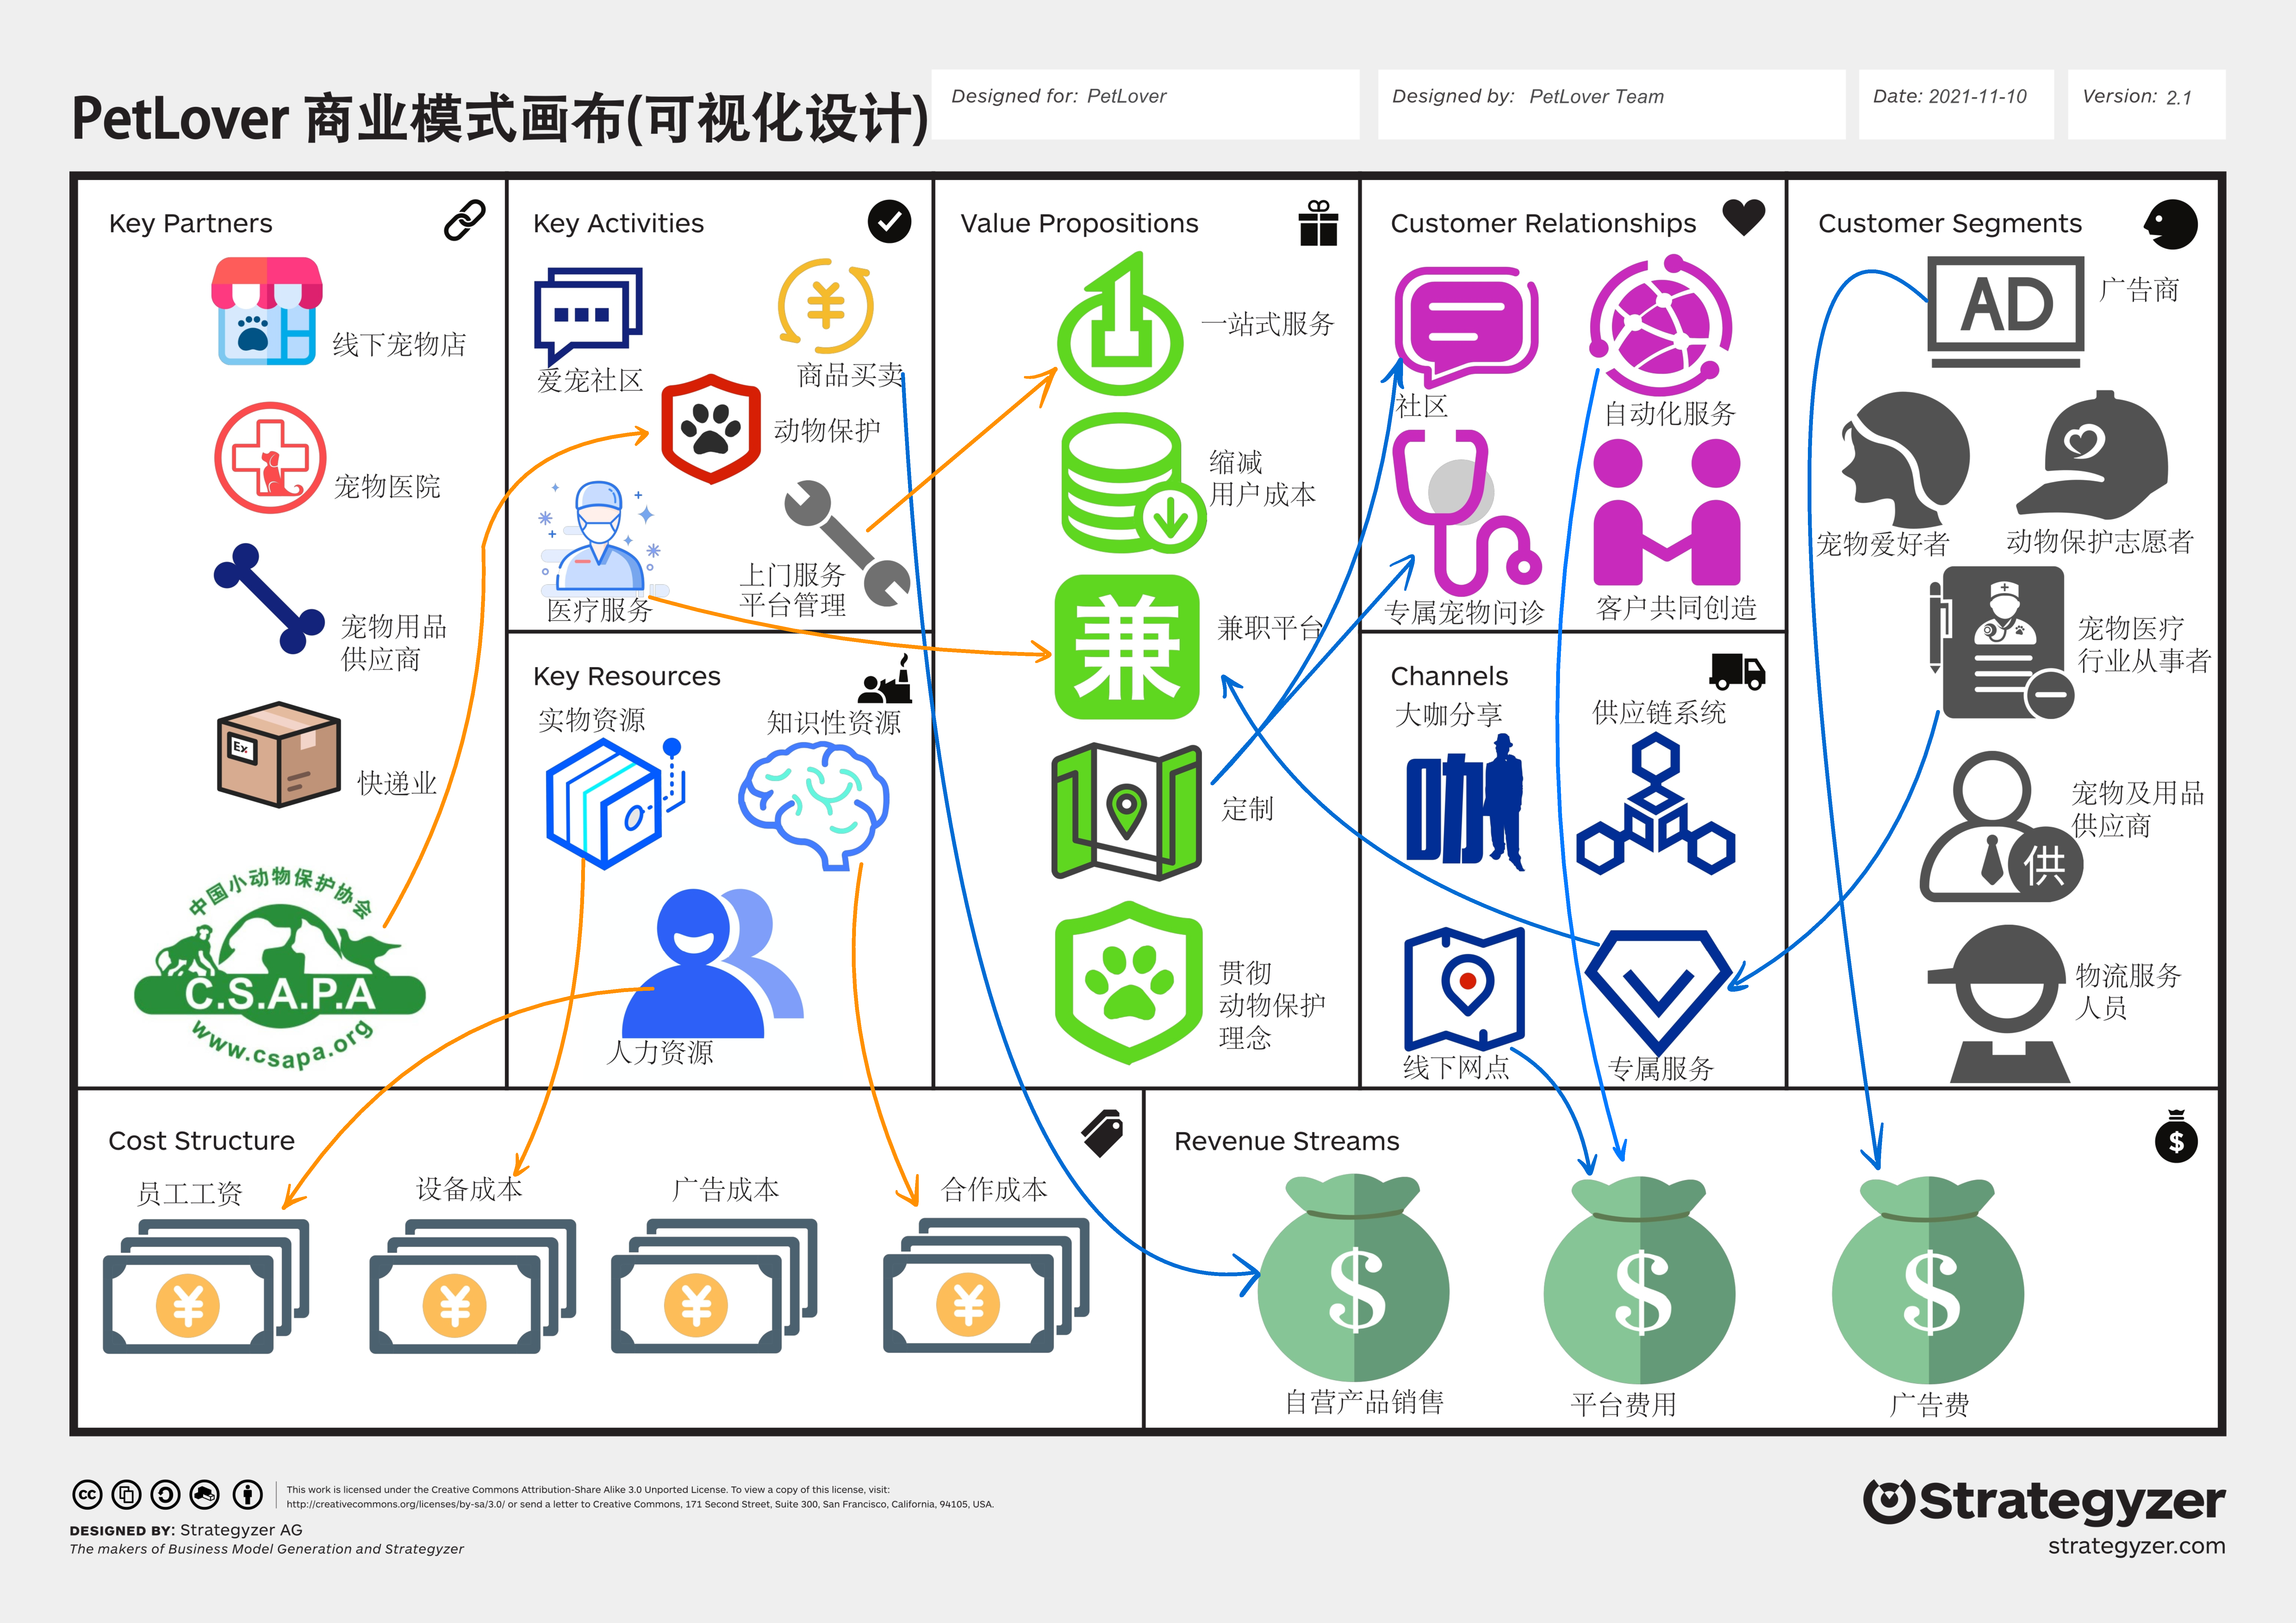
\includegraphics[width=16cm]{可视化画布v2.1}
\end{center}

\subsubsection{相关分析说明}

经过详细的讨论和落实,我们团队创建了一份可视化的商业模式画布(如上),建立了PetLover爱宠平台的大致商业框架。我们的业务核心是爱宠社区和商品买卖(宠物及宠物用品买卖),同时附加平台管理、医疗服务、商品买卖、动物保护等模块的业务。针对这些业务,我们对我们的客户群体进行了划分,其中占比最多的群体是宠物爱好者,他们是爱宠社区内容发布的主力军,其余群体分别为广告商、宠物医疗行业从事者、宠物及其用品供应商、物流服务人员、动物保护志愿者;价值主张以一站式服务(为宠物爱好者提供了宠物日常交流、宠物饲养教程、宠物及其用品购买、宠物健康咨询、宠物医疗服务便利的一站式服务,避免宠物爱好者在其他各个服务平台反复切换)为核心进行拓展,提供兼职平台、缩减用户成本、为不同用户群体进行定制社区、贯彻动物保护理念,打造一个博文内容、商品买卖可靠的大型宠物内容社区;客户关系也是以社区为纽带,为各类用户提供社区的自动化服务、专属的宠物问诊等,我们的团队同时与各类用户进行合作,共同创作平台内容,创造一种PetLover专属的社区文化氛围。PetLover以知识性资源为核心,其推广及经营的渠道通路广泛,包括大咖分享、供应链系统、线下网点、专属服务等,为资产销售、广告费用等收入来源提供了渠道,简化了项目的成本结构。

\subsection{模型构建}

经过我们对商业模式画布的反复修改和补充,我们最终建立了一个商业模型,模型阐述如下:

\subsubsection{商业模式画布}

\begin{center}
  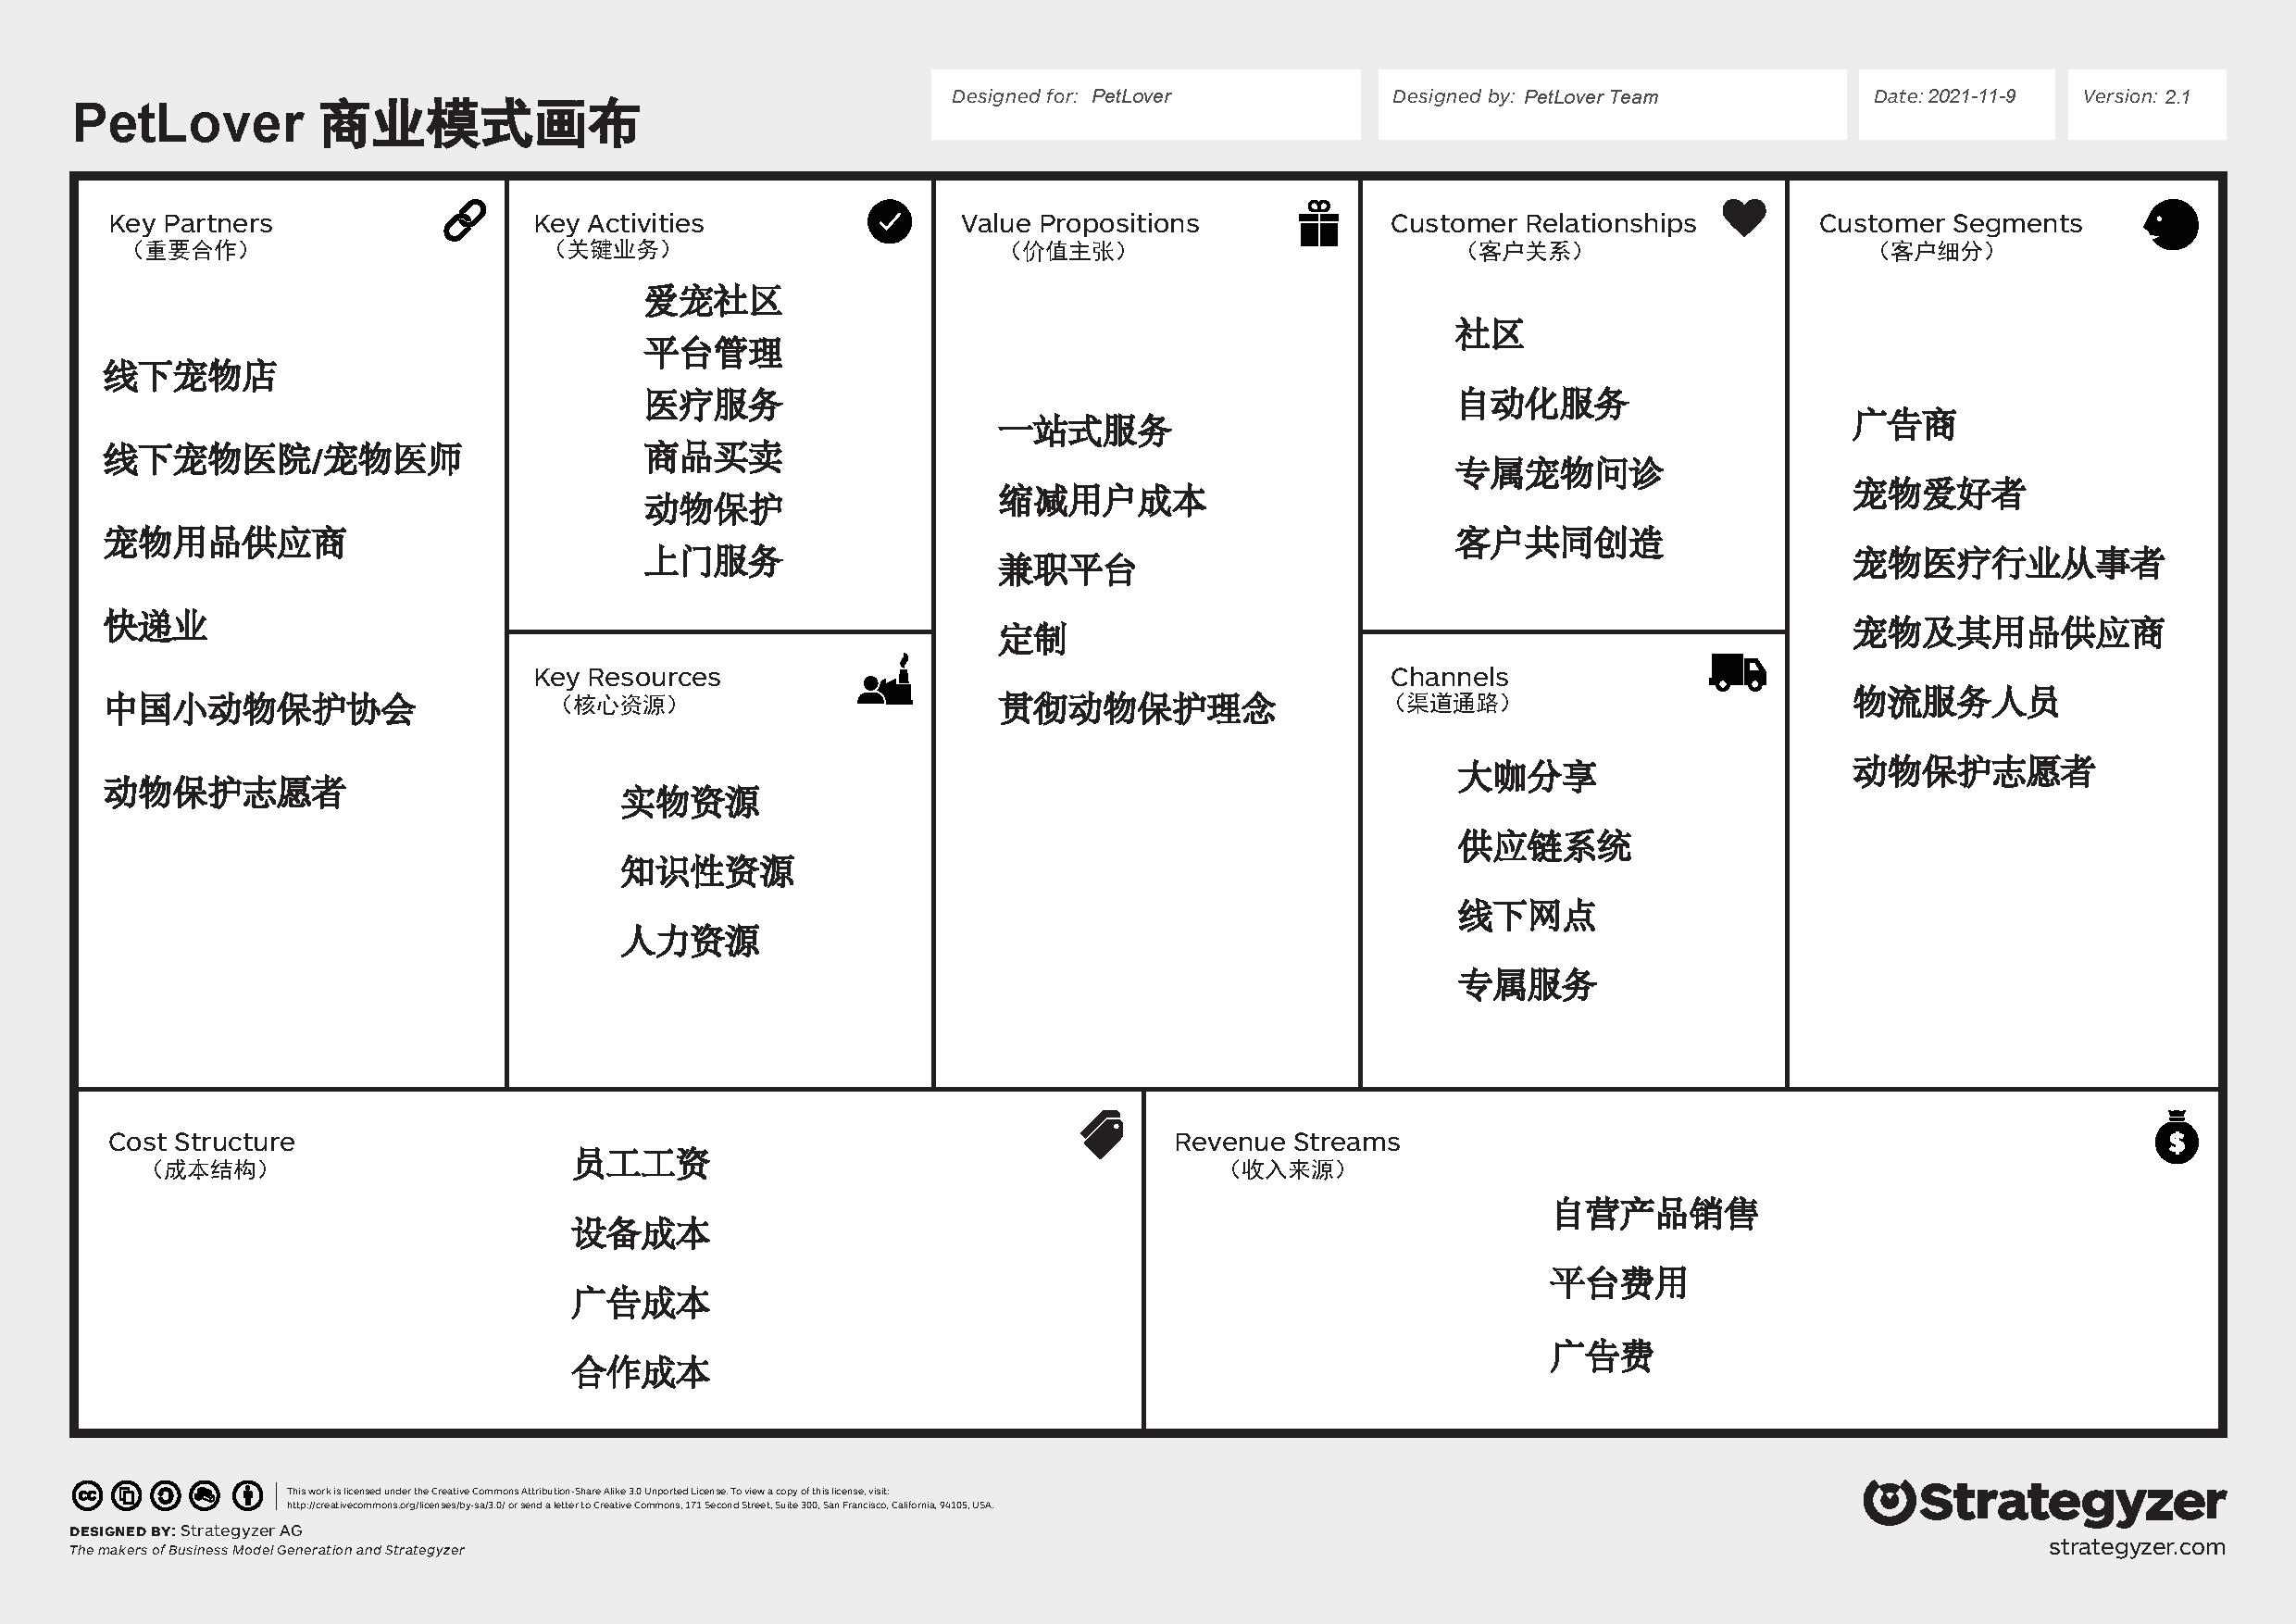
\includegraphics[width=16cm]{the-business-model-canvas1}
\end{center}

\subsubsection{市场潜力预估}

\paragraph{宠物行业背景概述:}
我国宠物行业从野蛮生长期进入了有序增长的稳定成熟期。我国宠物行业从20 世纪 90 年代初的花鸟市场年代,伴随着宠物消费产品和服务的日益丰富、人口结构的变化、宠物角色和养宠理念的转变、以及移动互联网技术对宠物行业交易模式和服务模式的改变,经过 30 年的发展,我国宠物行业经历了启蒙期、孕育期、快速发展期,目前进入了有序增长的稳定成熟期。
\begin{center}
  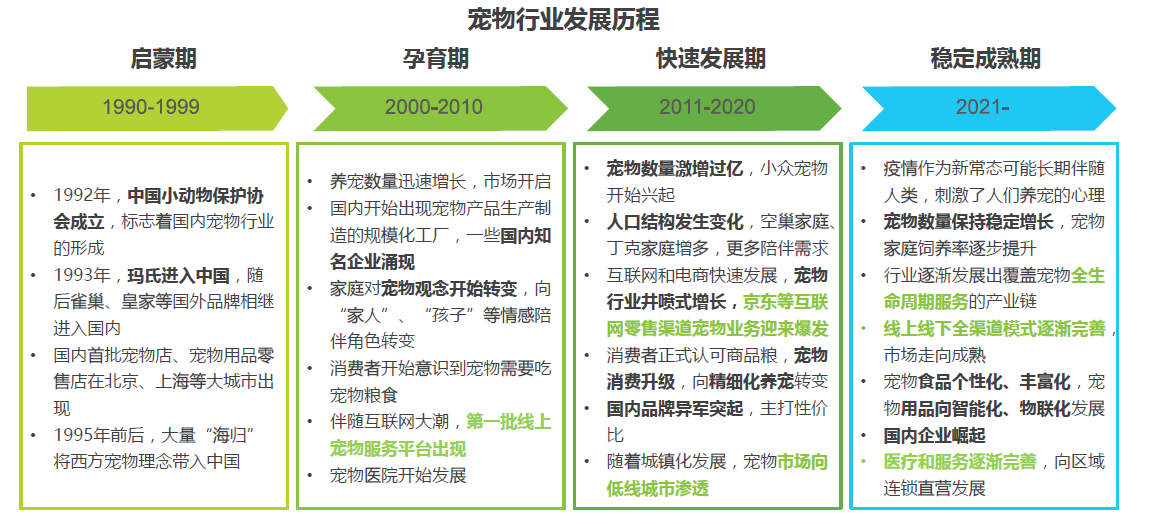
\includegraphics[width=16cm]{./assets/宠物行业发展历程.png}
\end{center}
宠物行业包括宠物交易和围绕宠物消费的商品和服务。宠物行业是指一切围绕着“宠物”而产生的产业链,涉及到宠物的繁殖与宠物交易,以及围绕宠物消费的商品和服务,包括宠物食品、宠物用品、宠物医疗和宠物服务。目前,我国宠物行业逐渐发展出覆盖宠物衣食住行、生老病死的全产业链。
\begin{center}
  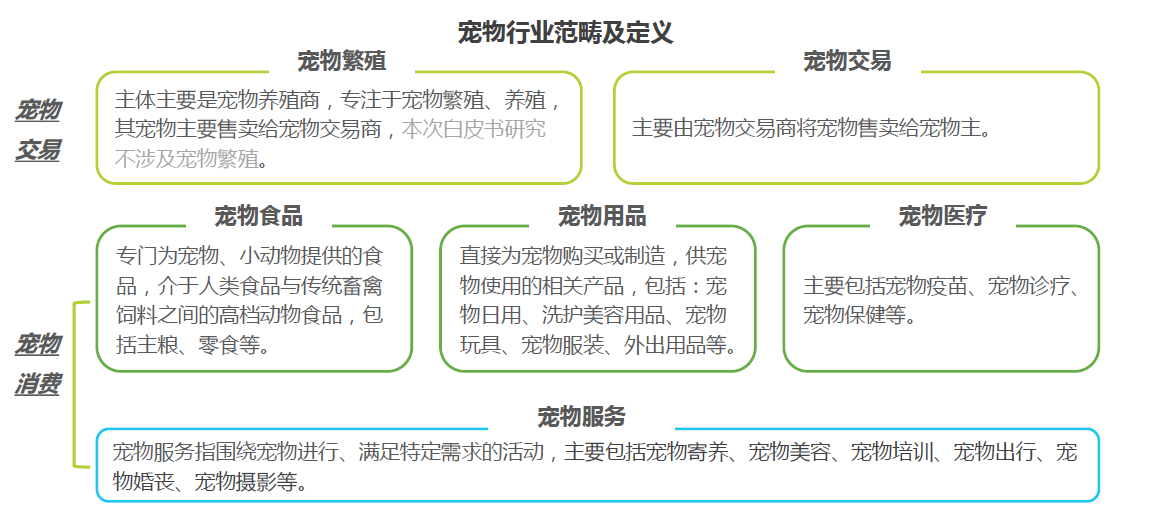
\includegraphics[width=16cm]{./assets/宠物行业范畴.png}
\end{center}
宠物行业产业结构以宠物食品是消费的核心,医疗、用品及各类型服务日渐增长。宠物食品类目是宠物行业最大的细分市场,随着人们对喂养商品粮的认知提升,市场对宠物食品的需求将进一步释放;其次是宠物医疗,主要为依托宠物医院和个体诊所的诊疗服务;宠物用品的细分品类较多,其中智能设备的成交量快速增长;宠物服务的形式日渐丰富,随着居民消费升级和养宠理念、宠物角色的转变,宠物服务行业将稳步增长。

\paragraph{宠物食品市场:}

当前,我国宠物食品行业仍处于较为分散的状态,国际品牌占据主要地位。华创证券资料显示,2017年中国宠物食品品牌份额(按零售价值)分布中,国际品牌占据超过百分之三十的市场份额。不能忽视的是当前国产宠物食品品牌的出现与发展,CBNDATA资料显示,2016年至2018年国产宠物粮食品牌销售额增速较快。至2020年,天猫双十一宠物品牌销售金额排行榜中,国产品牌占据5席。作为宠物市场最重要的细分市场,我国宠物食品市场处于高速发展的阶段,近几年平均增速保持在百分之二十左右。同时,基于我国供应链体系优势,新兴国产宠物食品品牌具备新生与成长的底层基础,但仍需品牌方夯实研发环节,注重满足宠物主对于宠物食品绿色、健康等需求的回应。

宠物食品市场产业链包括:食品研发-食品生产-食品销售等环节。其中上游食品研发环节以国内代工厂以及品牌自营研发基地为主;中游以宠物食品生产厂商为主;下游主要以宠物食品分销渠道为主,当前主要销售渠道包括商超、电商平台、便利店等。

PetLover平台参与宠物食品销售环节,要加强对中游的宠物食品生产厂商的密切合作关系,同时根据消费者对国产或者紧扣品牌的青睐程度作出市场调研,引进国内外的优质宠物食品产品,满足消费者的需求。

\paragraph{宠物医疗市场:}

在宠物医疗消费市场大型连锁宠物医疗集团已经出现,但医疗服务仍以个人宠物诊所为主。宠物医疗消费市场主要指代围绕宠物医疗需求的服务市场,通常包括疫苗接种、绝育、体检、门诊治疗、手术等服务。

当前市场中可以为宠物提供诊疗服务的线下机构包括宠物医院、个体宠物诊所、第三方检测机构、宠物店等。其中宠物医院是所有机构中专业性较强、诊疗手段较为先进的机构,通常可以为宠物提供门诊和手术、美容等多种医疗服务;个体宠物诊所是当前市场中数量最多的机构,以个人经营者为主。部分经营者持有兽医执照或会聘请具有兽医执照的兽医师参与经营活动,这类机构通常能够为宠物提供门诊、检测以及简单手术和美容、寄养等服务,相较于宠物医院的专业性,其综合性较弱,同时诊疗能力又高于普通宠物店;当前部分宠物店也会提供宠物诊疗服务,这种服务通常仅针对简单的病症;此外,宠物医疗市场中还有一类第三方检测机构也能够提供宠物诊疗服务,不过这种服务通常围绕动物样本检测展开。目前中国宠物医疗市场中以宠物医院、宠物诊所为主体,其中个体注册的宠物诊所是数量最多的机构。

PetLover平台提供专属的医疗服务希望能覆盖更加广泛的客户群体,因此平台不只需要为专业的宠物医院提供一个在线服务平台。个体宠物诊所作为一个广泛分布的,有空间局限性的,相对于宠物医院来说微小的可以整合的资源,PetLover能够为个体宠物诊所提供在线服务的窗口,让个体宠物诊所能够摆脱物理空间局限性,创造平台连接宠物爱好者与宠物医疗从业人员,最大化发挥优质资源的价值。

\paragraph{总结:}

随着我国宠物行业进入稳定期,宠物产业链不断完善,线上线下全渠道模式成熟,人们对于饲养宠物的需求不断增加,促使宠物行业市场标准化,专业化。但是目前宠物医疗市场、宠物服务市场等细分领域还存在着不足。PetLover瞄准当前定制化,一体式服务等高端服务需求,提供平台连接高质量服务者和客户。通过在线咨询、在线预约线下服务等方式,整合市场资源,节约客户成本,提升细分市场产品质量。同时通过用户创造内容的方式构建社区,每个细分客户分享优质内容,优质资源得以被发掘,既满足了宠物爱好者“云吸宠”的需求,又能够根据宠物爱好者对资源进行评估。

\subsubsection{商业模式画布要点}

本文档基于启动文档的商业模式画布做了如下几点修改:
\begin{enumerate}[label=\alph*.]
  \item 关键业务中增加了上门服务,这是我们在此次商业模式设计中进行创意构思整合后决定新加入的一个业务,包含对购置的大型宠物用品的上门组装/维修、同城线下宠物店爱宠送到家、宠物药品配送服务等,藉由此新添加的关键业务,能够更好体现我们的一站式服务和缩减用户成本的价值主张,并吸引更多潜在用户使用平台。
  \item 收入来源中的资产销售改为自营产品销售,平台支持宠物以及宠物用品交易,提供自营店与专卖店,掌握供应链,完善售后客服,提供一系列完整的消费服务,从中获取资产销售费用。
  \item 收入来源中的经纪人佣金改为平台费用,为了方便用户接受线下品牌实体店的服务,平台支持第三方宠物及其用品店交易以及宠物医院问诊,在服务过程中提供支付平台,从中收取交易手续费,同时平台费用会划分若干等级,根据等级调整向社区用户推荐购买链接和搜索出镜的概率。
\end{enumerate}

其余未修改的各个要点见画布,详细解释见启动文档。

\subsubsection{要点联系}

\paragraph{2.c(兼职平台)、3.c(宠物医疗行业从事者)、4.c(专属宠物问诊)、9.d(专属服务)}平台通过认证有从业资格的宠物医疗行业从事者进入平台,提供宠物健康在线咨询服务,收取咨询费用;作为兼职平台令宠物医疗行业从事者利用互联网互联互通优势,持续创造价值。
\paragraph{2.d(定制)、3.b(宠物爱好者)、4.a(社区)、4.d(客户共同创造)、9.a(大咖分享)}平台创造定制化社区,邀请养宠物的明星、网红等大咖入驻,提供高质量的社区内容,吸引更多的宠物爱好者反哺社区创造精品内容,不断吸引新的宠物爱好者进入,循换迭代扩大社区体量与质量。
\paragraph{2.a(缩减用户成本)、9.b(供应链系统)、9.c(线下网点)、3.d(宠物及其用品供应商)、3.d(宠物爱好者)}在线下网点与各个宠物及其用品供应商建立合作关系,对接平台物流,形成专属稳定的供应链系统。供应商进驻平台可获得优惠补贴,减少商家用户的经济成本。通过平台商品专门化集中化,通过平台自有供应链系统,减少宠物爱好者购买宠物商品的成本。
\paragraph{2.e(贯彻动物保护理念)、4.a(社区)、3.f(动物保护志愿者)}平台通过构建公益化的动物保护社区,吸引动物保护志愿者进入,让平台服务中心向外延伸拓展到动物。动物保护志愿者宣传动物保护,得到更多宠物爱好者支持,将理念传播到各个客户细分中。
\paragraph{2.a(一站式服务)、4.b(自动化服务)、4.c(专属宠物问诊)、9.b(供应链系统)、9.c(线下网点)、9.d(专属服务)3.d(宠物爱好者)}平台构建与宠物爱好者以自动化服务为代表的成本导向关系以及以专属宠物问诊为代表的价值导向关系,为宠物爱好者提供价格与价值优势。利用供应链系统、线下网点、专属服务渠道落实用户关系,实现一站式服务的价值主张。
\paragraph{6.b(线下宠物医院/宠物医师)、1.c(医疗服务)}通过与线下宠物医院/宠物医师合作,支撑起平台关键的宠物医疗服务,让宠物获得线上线下一体的医疗保障。
\paragraph{6.a(线下宠物店)、6.c(宠物用品供应商)、6.d(快递业)、1.d(商品买卖)}与各地区线下宠物店与其用品供应商建立合作关系,使用该平台作为线上宠物商品交易平台。同时加强与快递业合作,形成高效快速安全的物流网络,使得商品快速抵达提高用户使用体验。
\paragraph{6.e(中国小动物保护协会)、6.f(动物保护志愿者)、1.e(动物保护)}获取中国小动物保护协会的合作认证,吸引动物保护志愿者和自媒体入驻社区论坛。社区动物保护分区宣传动物保护思想,在法律允许的条件下可流浪动物领养公告,改善以宠物为主体的小动物生存条件,扩大动物保护公益事业。
\paragraph{5.b(知识性资源)、1.a(爱宠社区)、7.c(广告成本)}用户在社区中发表的精品内容是平台重要的知识性资源。在知识性资源的保障下,爱宠社区形成自己的专业知识壁垒,扩大爱宠社区影响力与知名度,形成社区资源的闭环扩张。为了打造资源富集的社区,需要投放广告来提升社区知名度,吸引优质知识性资源进驻平台。
\paragraph{4.c(专属宠物问诊)、9.d(专属服务)、8.b(经纪人佣金)}平台维系专属宠物问诊服务的价值导向关系,提供宠物医生专属服务渠道,从中收取经纪人佣金,使平台获得服务的高价值收入。
\paragraph{4.b(自动化服务)、9.b(供应链系统)、8.a(资产销售)}平台获取用户在社区浏览内容、饲养宠物类型、购买过宠物用品等信息,自动推荐用户潜在需要的宠物用品,以强大的自营或第三方知名宠物供应商的供应链系统作为渠道保证,获取资产销售收益,包括平台自营以及第三方平台中介费用。
\paragraph{4.a(社区)、3.a(广告商)、8.c(广告费)}平台通过用户体量庞大的社区,为广告商提供用户流量。平台允许优质的广告商以软广告推荐的方式进入社区,平台从中获取广告费用。
\paragraph{1.b(平台管理)、5.c(人力资源)、7.a(员工工资)}平台需要软件运维人员和平台与社区管理人员等人力资源,做到平台功能稳定、社区内容健康积极高质量、平台推荐商品质量有保障等平台管理关键业务。这样的人员工资开销构成了平台主要的成本开销。
\paragraph{1.c(医疗服务)、4.d(商品买卖)、5.a(实物资源)、7.d(合作成本)}为了维持平台的宠物医疗服务和宠物商品销售业务,平台需要宠物医院、宠物店、宠物用品供应商等线下实物资源来维护平台的资源壁垒和不可替代性。因此平台需要支付合作的线下实体资源优惠等合作成本来维护平台的不可替代性。
\paragraph{6.a(线下宠物店)、6.b(线下宠物医院/宠物医师)、9.c(线下网点)}平台需要加强和线下宠物店以及线下宠物医院/宠物医师的合作,才能通过实体设施维护和客户的线下网点的渠道通路良好运转。
\paragraph{6.c(宠物用品供应商)、6.d(快递业)、9.b(供应链系统)}平台把线下宠物用品实体店作为商品供应节点,与稳定的快递业合作形成商品快速流通网络,作为供应链系统的重要环节。
\paragraph{6.a(线下宠物店)、6.b(线下宠物医院/宠物医师)、6.c(宠物用品供应商)、6.d(快递业)、5.a(实物资源)}平台需要维持与宠物店、宠物医院/宠物医师、宠物用品供应商、快递业等重要合作,构建平台的实物资源,支持平台服务的稳定可靠运营。
\paragraph{2.a(一站式服务)、3.b(宠物爱好者)、2.c(兼职平台)、3.c(宠物医疗从业者)、8.b(经纪人佣金)}包含宠物健康咨询的一站式服务为宠物爱好者提供高价值私人服务;宠物医疗从业者进驻作为兼职平台利用零碎时间额外产生价值。平台通过这两个主张和客户细分从中获取经纪人佣金。
\paragraph{4.b(自动化服务)、8.b(平台费用)}平台在跟进用户需求进行自动化推荐服务的同时,会根据商家所付的平台费用(该费用会分若干等级)来调整向购买用品用户推荐相关链接的概率。
\subsubsection{支撑事实(新闻、调研及分析)}


\begin{enumerate}[label=\alph*.]
  \item 为什么宠物可以成为一个长尾投资趋势?
  \begin{enumerate}[label=\alph*.]
    \item 画布元素:核心活动,价值主张,客户关系
    \item 链接:https://www.morganstanley.com/ideas/us-pets-investing-trend
    \item 内容概要:疫情后的美国的宠物产业现状分析以及未来宠物产业细分市场
    \item 分析:疫情已经颠覆了人类的生活,但对于宠物来说,却是一笔财富:它们的主人一整天都在家里,时时刻刻都在关系和照顾它们。2021年的一项调查发现,百分之六十六的美国家庭至少拥有一只宠物,平均 1.7 只。大部分的受访者“强烈同意”他们的宠物是家庭的重要成员,约三分之一的人会借债来支付宠物的医疗费用,约百分之三十的人会把宠物的需要放在自己的前面。同时,宠物主人——尤其是年轻的主人——在他们的宠物上花费越来越多。通过这样的事实证明,即使在经济处于衰退期间,从兽医护理到宠物配件的所有支出都具有弹性的,人们愿意为宠物支出。除了宠物的“衣食住行”,越来越多的人会关注宠物的健康。在宠物食品和零食之后,动物健康是最大的细分市场,而宠物护理可能是宠物行业未来十年增长最快的细分市场。PetLover平台提供包括宠物食品购买、宠物医疗服务等的一站式服务,涵盖了当下与未来宠物行业的热门细分市场,立足于当下的增长点,发展未来宠物医疗的可能性。
  \end{enumerate}
  \item 中国宠物行业的异军突起背后的问题
  \begin{enumerate}[label=\alph*.]
    \item 画布元素:重要合作
    \item 链接:https://pandaily.com/the-extraordinary-rise-of-chinas-pet-industry/
    \item 内容概要:宠物行业的进入门槛低以及宠物行业的相关政策法规的法律空白导致宠物行业出现许多问题。
    \item 分析:根据中国社交网站狗民网(Goumin.com)和亚洲宠物博览会(http://www.petfairasia.com/)联合发布的《2020中国宠物行业白皮书》,2020年城市居民饲养的猫狗数量达到10084万只。中国城市常住人口接近8.5亿,这意味着十分之一的人拥有一只宠物猫或狗。宠宠的热潮,促使许多垂涎宠物经济带来的丰厚利益的投资者,急切地进入这个行业,争先恐后地在蓬勃发展的市场中分一杯羹。近年来,宠物美容、宠物寄养、宠物运输等宠物相关服务如雨后春笋般涌现。大量投机者涌入宠物行业,其中大部分没有接受过专业培训,宠物服务质量参差不齐。填补宠物行业的相关政策法规的法律空白来使得宠物行业标准化的到来可能还有很远一段路要走,PetLover平台通过对重要的合作者,例如宠物医院,线下宠物店,快递业等的资格认证和服务质量要求,提供高于法规的标准,信誉有保证,专业周到的宠物产品和服务,有效地缓解宠物行业相关法律法规不完善的问题,保证服务质量。
  \end{enumerate}
  \item 《2020年中国宠物行业白皮书》发布,宠物行业迎来“千宠千面”新食代
  \begin{enumerate}[label=\alph*.]
    \item 画布元素:客户细分,价值主张
    \item 链接:http://www.forbeschina.com/business/55094
    \item 内容概要:《2020年中国宠物行业白皮书》发布,揭示中国的宠物行业新的发展趋势
    \item 分析:据《2020年中国宠物行业白皮书》显示,2010年以后,国内宠物行业进入快速发展期。伴随着国内养宠方式的转变和宠物角色朝着伴侣方向的变化,宠物的家庭属性和地位逐渐稳定。大部分的宠物主人将宠物视作自己的孩子或家人。人均收入提高、消费升级以及养宠观念发生转变,宠物与人的感情黏性增强等因素驱动,宠物服务行业逐渐兴起,宠物市场空间迅速扩大。同时,我国宠物行业上升空间巨大。我国的宠物饲养率与发达国家相差较大,未来宠物数量仍然有很大的上升空间;宠物消费不断升级,单只宠物消费额逐年上升。电商经济推动宠物食品行业爆发式增长,各种品牌的宠物食品百花齐放,逐渐进入“千宠千面”的定制化阶段,开启了“新食代”。PetLover平台主张定制化,为我们的主要客户细分——宠物爱好者,提供更加定制化专门的宠物建议,从饮食到医疗再到宠物产品,从多方面进行定制化。
  \end{enumerate}
  \item 高盛表示中国的宠物护理支出将大幅增加
  \begin{enumerate}[label=\alph*.]
    \item 画布元素:收入来源,价值主张,客户关系
    \item 链接:https://www.ft.com/content/d9b76550-bd18-4f1a-acf1-68fb6616cd65
    \item 内容概要:高盛表示中国宠物市场将持续扩大,随着每只宠物支出的不断扩大,宠物行业收入将不断上升。
    \item 分析:高盛投资银行在一份 104 页的报告中阐述了中国宠物护理市场的案例。该报告预测,从现在到 2030 年,宠物食品支出的年复合增长率将达到百分之十九,因为除其他因素外,中国有近2亿只猫和狗从吃剩菜转向吃包装宠物食品。至关重要的是,该报告预测未来十年中国宠物市场将发生转变,因为该行业正在扩张以满足快速增长的单身和老年人口的需求。高盛说,这两个人口群体与每只宠物的支出都比世界其他地方更高。PetLover平台构建宠物社区,利用用户创造内容(UGC),为单身以及老年人为代表的宠物爱好者提供更加优质的宠物饲养体验,能够在自己饲养宠物的同时,接收其他宠物爱好者的分享信息,沟通饲养心得,结识同道“宠友”。PetLover留住高价值客户,创建潜在的消费场景,从而在不断扩增的宠物行业中获取客观收入。
  \end{enumerate}
  \item 持续加强合作,让苹果越走越远
  \begin{enumerate}[label=\alph*.]
    \item 画布元素:重要合作、渠道通路、核心资源
    \item 链接:https://www.sohu.com/a/477844359\_120651198
    \item 内容概要:苹果与京东方展开合作,苹果设备屏幕供应链再添得力帮手
    \item 分析:苹果作为全球单品出货量最高的手机品牌,每年都有数亿计的苹果产品问世、售出,其对供应链的要求之高可想而知。仅以手机屏幕来说,它是用户使用手机时直接进行交互的媒介,重要性不言而喻,由此苹果公司从初期逐渐扩大合作范围,逐渐与康宁、LG、三星、Japan Display、夏普等屏幕供应商展开合作,保证了屏幕产量充足,而据2021年7月消息报道,苹果又与中国厂商京东方携手合作,并且京东方专门为苹果独家定制实验性产线。可见,对于一款期望长期稳定发展的产品,与第三方合作者达成良好的合作关系是十分关键的一环,能够使产品持续健康发展。
  \end{enumerate}
  \item Cambly——让大众也能体验纯正外教英语课
  \begin{enumerate}[label=\alph*.]
    \item 画布元素:收入来源、客户关系
    \item 链接:https://zhuanlan.zhihu.com/p/282818682,https://www.douban.com/note/734581924/
    \item 内容概要:Cambly 虽然日常价格较为昂贵,但其周期性的营销活动和折扣让普通学生也能以合适价格体验到和英语母语者的交流机会,并不断提升自己的英文水平
    \item 分析:一款基于资源驱动和客户驱动的英语口语练习软件 Cambly,其提供了优质的外教资源,包括来自于美国、英国、澳大利亚等多个母语国家的外教,提供不同类型的课程。但该软件课程费用较为昂贵,导致面向用户数量较少,为了吸引新老用户购买课程,该软件采用了邀请码和课程折扣等机制,被邀请者和邀请者都可获得一定时间的免费试听课,根据需要选择喜欢的外教继续购买课时;每逢节日,课程都会推出一定折扣,甚至会达到三八折,可能让那些先前被价格“劝退”的英语学习者选择购买。由此,我们的 PetLover 平台也应该视情况定期推出相关活动,以客户驱动创新,不断吸引新用户前来加入平台。
  \end{enumerate}
  \item 萌牙家?猛牙家!一款专注于“打广告”的电动牙刷
  \begin{enumerate}[label=\alph*.]
    \item 画布元素:成本结构、重要合作、渠道通路
    \item 链接:https://zhuanlan.zhihu.com/p/66738348,https://www.zhihu.com/question/67870993,https://zhuanlan.zhihu.com/p/56566708
    \item 内容概要:萌牙家广告投放合作分析及相关差评反馈
    \item 分析:一款十分注重广告和合作的产品——萌牙家电动牙刷,给人一种“一夜爆红”的感觉。具体体现为各大(短)视频平台中短时间涌现出大量推荐这款产品的合作博主,让广大观众“猝不及防”,此外还有微博博主进行宣传和撰写软广文,即使是从未使用过或听说过这款产品的用户,在经过了视频“安利广告”和博主推荐后,也对这款产品产生了深刻的印象,萌牙家电动牙刷销售额节节攀升。但过多的广告一定程度上会让人对产品产生反感,虽然将产品品牌打了出去,但我们发现,该款牙刷的实际使用反馈评价并不好(如已购用户对于产品质量、售后等方面均有不少差评),我们认为可能是该款产品在广告成本上投入过多、用力过猛导致的。因此在均衡成本结构时,更要充分考虑财务的分配,保证平台正常运转的同时,达到积累用户、创收更多、口碑更好的目的。
  \end{enumerate}
  \item 中国小动物保护协会CSAPA——贯彻动物保护理念
  \begin{enumerate}[label=\alph*.]
    \item 画布元素:重要合作、价值主张
    \item 链接:(https://mv.lingxi360.com/m/z0jvzv?utm\_bccid=LXEsJeJt)
    \item 内容概要:CSAPA(中国小动物保护协会)让我们一起爱护小动物
    \item 分析:中国小动物保护协会是国家一级专业性社会团体,以珍爱生命、倡导精神文明和发扬人道主义精神为思想基础,以保护动物、维护动物的生存权利和不受虐待的权利、以及改善和提高小动物的生命条件、饲养水平为宗旨,坚决反对任何虐待、残害动物的行为和思想。他们所倡导和宣传的动物保护理念也是我们PetLover平台的初心和矢志不渝坚持的目标。我们还发现:在他们的宠物领养页面中,关于待领养宠物的信息,只会了解到宠物们的年龄、性别、性格等大体信息,而不会知道它们的具体品种——有些一昧追求纯种宠物的人对所谓的“田园犬”毫无爱心可言。CSAPA真正地让我们看到了爱护小动物带给人间的一份温暖,这也将鼓励我们平台坚持走下去。
  \end{enumerate}
  \item 2021宠物医院行业现状如何 未来宠物医院的发展趋势分析
  \begin{enumerate}[label=\alph*.]
    \item 画布元素:关键业务、客户细分、渠道通路
    \item 链接:https://www.chinairn.com/news/20210615/15570027.shtml
    \item 内容概要:文章分析了国内宠物医疗行业的发展现状以及未来的发展趋势,阐述行业整合将成为宠物医疗企业持续发展的重要手段的事实。
    \item 分析:中国宠物爱好者是一个庞大的群体,人们对宠物相关服务的需求不断扩大,宠物医疗行业发展必不可少;但是当前中国宠物医疗行业整体运行处于低水平状态,虽然从事这项工作的机构很多,但大多数经济实力不强、技术水平较低、资金分散、规模小、效益低。而且地域差异较大,表现在宠物医疗机构在一二线城市分布密集,在小城市或农村地区分布较少,大多处于中心城区,社区周边和街道较少。宠物医疗行业应当同互联网相结合,使用互联网作为发展平台,进行资源整合,拓展业务范围、扩大网络布局。而PetLover平台为宠物医疗行业从事者提供了这样的平台,同互联网结合,消除地区差异和资源分散带来的行业弊端。
  \end{enumerate}
  \item 宠物社区是否有成立的可能?
  \begin{enumerate}[label=\alph*.]
    \item 画布元素:关键业务、客户关系、渠道通路
    \item 链接:http://www.woshipm.com/it/3368333.html
    \item 内容概要:作者在宠物领域创业一年,思考了宠物社区是否有成立的可能,从市场横向进行分析对市场的垂类进行研究,提出了几点个人想法
    \item 分析:尽管很多类似微博的新媒体平台宠物内容占比较高,但宠物领域一直没有看到一个有影响力的社区出现。目前宠物行业的发展情况有如下几点:养宠人群基数足够大、国内宠物市场发展快但起步晚、国内用户对于养宠的消费升级意识在逐步提高。而且当今养宠群体分为初级型、中级型、进阶型三类,晒宠、购物、科普和养宠讨论都会由这三大群体共同完成,这些活动都需要社区这种土壤来培养,随着宠物社区的成长,养宠或许在未来成为人类生活重要的一部分。因此,宠物社区的出现和发展是一个大趋势,它或是像微博超话一样寄居式生长,或是如我们PetLover项目提供单独社区独立式生长。文章最后提到了宠物消费问题和宠物服务问题(医疗服务、生活科普服务)对于养宠用户的社区来说是绕不开的大山,如何处理好宠物消费、科普和社区的关系是社区搭建中一个比较重要的问题。
  \end{enumerate}
  \item P出世界的精彩?小红书变“小黑书”,造假终究成不了财富密码!
  \begin{enumerate}[label=\alph*.]
    \item 画布元素:价值主张、渠道通路、重要合作
    \item 链接:https://www.163.com/dy/article/GN2OO3QD0511BMPU.html
    \item 内容概要:文章主要阐述了小红书商业模式的走偏,分析了小红书的造假行为,对已经被搞乱的小红书来说,当信任被透支,唯一的腿被折断,那就不是道歉能解决的问题了。
    \item 分析:在当今互联网时代,信息洪流不断冲击这广大网民,信息真实性的辨认成为了让网民头疼的问题,在这种环境下网民选择使用信誉度高的平台而丢弃丧失信誉的平台,互联网时代造假成不了财富密码。对于小红书,曾以“记录真实生活”作为口号,如今却成为造假、失真的“摇篮”,令人唏嘘。当一个种草社区无法种草,信任被透支后,可不是一两句道歉能挽回的事。我们的PetLover作为创业初创项目深刻的思考了这个问题,PetLover在社区方面的商业模式设计与小红书类似,但在价值主张、渠道通路和重要合作中与小红书有所不同,我们要求宠物及其用品供应商供应一定可靠,质量有所保证,且进驻本平台的广告商、电商的经营许可证、产品合格证、经营方式、范围都要经过严格把关,保证平台的信誉,为用户提供一个纯净的平台。
  \end{enumerate}
  \item 2021年中国宠物饲料行业产业链分析:居民饲养宠物市场规模不断扩大,宠物食品需求大幅增加
  \begin{enumerate}[label=\alph*.]
    \item 画布元素:重要合作、关键业务
    \item 链接:https://xw.qq.com/amphtml/20211101A03L8300
    \item 内容概要:我国宠粮品牌发展逐渐趋于好转,尤其是在线上渠道充分发挥出了优势。
    \item 分析:全球宠物市场已逐步成熟,宠物食品作为宠物行业的一个重要分支,是宠物市场最大的“蛋糕”,全球宠物食品市场占整个宠物行业的比重逐年增加。2020年全球宠物饲料产量为29.3百万吨,较2019年的27.7百万吨同比增长百分之五点八。随着中国宠物经济的崛起,宠物食品行业受到了越来越多的关注,宠物食品是保障宠物健康的基础,人们对宠物食品的追求逐渐与人类食品趋于一致,预防性和主动性健康措施已成为消费者最看重的问题。近年来,中国宠物饲料行业产量及需求量不断增加,根据中国饲料工业协会数据:2021年1-8月中国宠物饲料产量为62万吨,较上年同比增长百分之十三点五。PetLover可以发挥电商平台的关键作用,建立高质量宠物食品买卖的供应链系统,促进宠物周边消费,打造全方位宠物社区。
  \end{enumerate}
  \item 宠物经济行业:2020年中国四成宠物主关注宠物APP的社区交流
  \begin{enumerate}[label=\alph*.]
    \item 画布元素:关键业务、价值主张、渠道通路、客户关系
    \item 链接:https://baijiahao.baidu.com/s?id=1676168006448060521\&wfr=spider\&for=pc
    \item 内容概要:宠物app的社区化将成为主流。
    \item 分析:艾媒咨询数据显示,2020年2月份淘宝宠物直播场次同比增长百分之三百七十五,每天观看人数超100万。疫情期间云经济快速发展,“云吸宠物”模式更加成熟,也从以往看图说话、视频逗趣的形态升级为24小时超长直播、隔屏互动,充分体验“云养宠物”。可以预见,疫情结束后,“云经济”将以更具爆发力的形态发展。PetLover可以充分利用其自身爱宠社区的优势,打造良好的社区环境,增强用户粘性,提高用户留存率。
  \end{enumerate}
  \item 中国宠物电商行业研究报告发布,看播次数增长百分之一百八十六,宠物达人和品牌企业积极开播
  \begin{enumerate}[label=\alph*.]
    \item 画布元素:关键业务、渠道通路、收入来源
    \item 链接:https://www.thepaper.cn/newsDetail\_forward\_14079967
    \item 内容概要:《中国宠物电商行业研究报告》发布,分析了数个品牌案例,指出了中国宠物电商行业的发展趋势。
    \item 分析:中国宠物电商市场规模在过去五年里迅速增长,2020年我国宠物电商市场规模接近300亿元,2015-2020年间复合増速达到百分之三十八点八。尤其在疫情期间,萌宠内容获得爆发式关注,加速了在线“云吸宠”人群的扩张,培养了更多新的潜在消费者。同时,大量国际和本土宠物品牌都已开启了在短视频平台的品牌阵地布局,直播带货进入常态化经营阶段。从户均宠物数量来看,现阶段我国养宠渗透率显著低于美国、澳大利亚等国家,意味着我国宠物电商市场仍有巨大增长空间。随着养宠规模的扩大、相关政策的助推以及直播短视频发展的驱动,我国宠物电商赛道将迎来进一步升级。PetLover可以在宠物电商赛道加大投入,在宠物垂直电商领域中挖掘低线市场潜力。
  \end{enumerate}
  \item 宠物电商:针对宠物人群的电商结构思考
  \begin{enumerate}[label=\alph*.]
    \item 画布元素:关键业务、渠道通路、收入来源
    \item 链接:https://baijiahao.baidu.com/s?id=1685142650486617920\&wfr=spider\&for=pc
    \item 内容概要:宠物行业已经形成了千亿级市场,围绕其诞生的相关子行业也在不断发展
    \item 分析:宠物行业规模已破千亿,但这一垂类尚未形成有明显优势的国内品牌;在宠物服务领域,在线诊疗、宠物寄养、宠物保险等也存在一定缺口。对于宠物电商来说,宠物主人对于电商的需求,一是在于专业权威、正品保障,通过平台能快速了解养宠信息和商品测评;二是价格优势;三是购物流畅度,商品能匹配宠物特性进行分类、品类覆盖全、购买省时省心。PetLover的主要优势在于社区+电商。社区的主要作用是承担流量入口、用户留存以及向电商板块的转化,需要加强与电商板块的连接。
  \end{enumerate}
\end{enumerate}

\subsection{讲故事}

为了形象生动地呈现PetLover的商业模式,我们总共构建了5个故事来帮助理解。其中4个是用户视角的故事,1个是公司视角的故事。

\subsubsection{宠物爱好者}
晓琳是一个宠物爱好者,她一直都很想拥有属于自己的猫咪。大学毕业后,她找到了自己喜欢的工作,挣到了人生的第一桶金。正当她拿着钱打算去宠物店买一只小奶猫的时候,她却犹豫了,理由是她妈妈认为养宠物不仅要花很多钱,而且麻烦不卫生,需要做好准备。

她确实非常非常喜欢猫咪,但她也觉得妈妈的担心不无道理。对晓琳来说,在养宠物这件事情上,说服自己貌似比说服妈妈更加关键。为了让自己能够做好充足的准备来迎接自己人生中的第一只小猫咪,晓琳费尽心思在各种社群平台上搜索养猫攻略,但都以内容过于分散无法形成体系而草草收场。她只好在暂时在不同的平台上进行“云吸猫”,关注一些”明星“猫咪,来满足自己心理上对猫咪的强烈需求。

想养好猫咪,你最好能有一个万全的”铲屎官“攻略。这也是为什么当晓琳通过”云吸猫“发现PetLover的时候(渠道通路——大咖分享),她就被深深吸引了。PetLover正好解决了晓琳的几个重要工作:海量养猫达人分享的完整养猫日记(关键业务——爱宠社区),电商平台上官方出售的高质量猫粮与日用品(关键业务——商品买卖),以及品牌宠物医院提供的无忧问诊服务(关键业务——医疗服务)。这也正是PetLover平台的几大核心板块。

得益于PetLover的一站式服务(价值主张——一站式服务),晓琳很快就做好了充足的准备工作,并拥有了人生中第一只小奶猫。晓琳再也不用在如何养猫这件事情上伤脑筋,她只需要简单地按照PetLover上的全方位攻略(价值主张——缩减用户成本),使用它提供的资源(知识性资源),就可以非常轻松地养好小猫咪。跟之前所担心的恰恰相反,她发现养小猫咪一点都不麻烦,而且家里甚至比以往更加干净整洁了。

养了小猫咪之后,晓琳的生活变得丰富起来。她又新买了两只小猫咪,养猫成了她的快乐源泉。晓琳把每天拍下来的小猫咪们的素材也分享到了PetLover上(客户共同创造、社区),可爱的小猫咪搭配漂亮的小姐姐,让晓琳收获了不少的点赞和关注。她现在已经有了小几万的关注量,也算得上是个知名宠物博主了(客户关系——客户共同创造)。
\subsubsection{宠物医疗行业从事者}
阿添是一个宠物医生,毕业于兽医专业的研究生,现在在一个三线城市的宠物医院工作。这家宠物医院平时的客流量很小,阿添每天接待的”病人“屈指可数,因此日子过得十分清闲。

虽然这份工作朝九晚五而且比较轻松,但是宠物医生的收入并不高,所以他萌生了在下班之后或者双休日的时候兼职赚点零花钱的想法。他在几个平台上注册了兼职医师,想利用自己的专业知识做宠物医疗线上咨询。但很遗憾,他发现这些平台的客流量跟他所在的宠物医院大差不差,一天下来基本没多少人提问,所以兼职的收入也并不可观。

正当他感慨宠物医疗受众面窄的时候,他所在的宠物医院与PetLover达成了合作(重要合作——宠物医院),在院内邀请医生担任线上咨询医师,阿添第一个就报了名。入驻PetLover后,阿添惊喜地发现这个平台的客流量很高,每天各个宠物主人提出的问题令人目不暇接。这恰恰是阿添所需要的——大量的客流量所带来的可观的收入(价值主张——兼职平台)。他再也不需要在好几个平台之间切换来苦苦寻找有没有宠物主提出新问题,只需要盯着PetLover的医疗服务咨询板块,在上面的海量问题中挑出自己熟悉的领域进行精准而恰到好处的讲解(客户关系——专属宠物问诊)。

阿添马上就明白了为什么PetLover可以解决他的烦恼。这家平台不仅仅是一个线上医疗咨询平台(关键业务——医疗服务),还整合了宠物日常分享、宠物饲养攻略(关键业务——爱宠社区)、宠物用品买卖(关键业务——商品买卖)等功能。PetLover以它的多渠道跨界整合,发挥社群+电商的模式,吸引了大量用户。平台日活量高、用户粘性强,因此给医疗服务咨询板块带来了大量的流量。

现在,阿添每天下班之后都积极回答宠物主人们提出的问题。看着他通过自己的努力给宠物主人们答疑解惑、让生病的宠物们恢复往日的活力,他的心里充满了成就感。随着他在平台内的活跃度与权威度越来越高,他也接到了不少用户定制的专属服务,在一对一提供专业治疗建议的同时,还持续跟进后续治疗,宠物主人们都十分满意(渠道通路——专属服务)。还有不少宠物主人慕名而来,专门跑到他所在的宠物医院登门问诊(渠道通路——线下网点)。通过PetLover的兼职医师,他的收入跟以往相比几乎翻了个倍呢。
\subsubsection{宠物及用品供应商}
小川是一家宠物用品商店的老板,经营着一家规模中等的宠物用品实体店。小川的经营理念是以质量取胜,他的宠物用品商店在当地有着十分不错的口碑,在他们家买过宠物用品的宠物主人们基本都会成为他的回头客。

小川不止一次想过扩大自己的经营规模,他投向电商平台,在天猫上开了一个网店。但网店需要收较多的广告费来进行推广,同时他也没有时间精力亲自邮寄自己的商品。网店开了一段时间后,出于发货慢和推广不足等原因,他的网店的评价一直不是很好,所以他放弃了网店的运营。

去年一个偶然的机会,他的一个养宠朋友给他推荐了PetLover平台。小川得知平台上面入驻了不少宠物用品商店,但是他们所在城市并没有宠物用品店的线下网点,于是果断联系PetLover平台入驻。在交了一笔相对不高的加盟费后(收入来源——平台费用),小川所经营的宠物用品商店成为了当地第一家PetLover的线下网点(重要合作——宠物用品供应商、重要资源——实物性资源)。同时,小川所经营的宠物用品商店的网店也在PetLover上重新开始经营(关键业务——商品买卖)。

由于小川的实体店是平台认证的官方线下网点(渠道通路:线下网点),很多当地的PetLover用户纷纷前来采购,而小川的商品质量也确实是名不虚传。实体店本就不错的口碑配合平台的认证,让宠物主人们彻底放心,大家都愿意来光顾他们家的店,让实体店的销售额与日俱增。而同时,小川的网店也做得红红火火。得益于PetLover平台完善的物流服务(重要合作——快递业),小川再也不用烦恼自己的商品的邮寄问题了,也降低了他网店经营的成本,又取得了不错的口碑。

现在,小川所经营的宠物用品商店可以说是线上线下两开花。他的线下实体店已经在当地开了好几家连锁店(渠道通路——供应链系统),并正在往周边城市发展。而他的线上网店由于商品质量有保证,被平台评为十佳宠物用品商店。一年前,小川做梦也没想到,自己的小店能够发展到今天的规模。
\subsubsection{动物保护志愿者}
淑元是中国小动物保护协会的一员,也是一个热心的动物保护志愿者。她常年奔波与动物保护公益事业,致力于小动物救助与领养。这不,她自己家里就领养了十几只流浪猫,在她的悉心照顾之下,小猫们都非常健康。

平日里,淑元也经常向她的亲戚朋友邻居同事们宣传小动物保护的思想,号召大家保护流浪动物、发扬人道主义精神。但是,靠她一个人的力量,这种宣传方式收效甚微,本地的流浪动物状况完全没有得到改善。况且,她的宣传对象们大多都没有耐心听她宣传,能听进去的也几乎不会帮她进行二次宣传,她只好另谋出路。

很快,她就注意到了与中国小动物保护协会合作的PetLover(重要合作——中国小动物保护协会)。该平台获得了中国小动物保护协会的授权,且平台本身十分注重动物保护理念,动物保护者们可以入驻社区,宣传动物保护的思想(价值主张——贯彻动物保护理念)。她随即就注册了一个账号,通过了动物保护志愿者的认证,并以志愿者的身份发布了一些关于当地小动物保护的推文(关键业务——动物保护)。

很快,她的推文就收到了上万的浏览量。淑元发现,这个平台上面的社区是宠物交流社区(客户关系——社区),大家都对小动物有着共同的喜爱。因此,在这个平台上进行小动物保护的宣传,无需东奔西走,就有着非常精准的受众(关键业务——爱宠社区)。这也是为什么她的推文能受到如此高的关注,这是以往她从未设想过的宣传效果。

果然,没过多久,当地的宠物医院与流浪猫救助协会联系上了淑元,邀请她一同参与正在进行的小动物救助的项目。淑元看到情况正在渐渐地变好,心里乐开了花。

\subsubsection{公司视角}
PetLover的创始人小刚,南京大学软件学院毕业,具有十年互联网从业经历。小刚自己养狗有六年,也算得上资深的宠友,说到怎么想到创立PetLover的时候,还要从发生在他家狗狗身上的两件事情说起。

第一件事:狗狗怀孕了怎么办?前两年,他家狗狗怀孕了。由于是狗狗第一次怀孕,所以完全没经验,不知道应该吃什么,能不能洗澡等等。身边养狗的朋友说法不一,只能到网上去搜索相关内容。不过让他郁闷的是:网上的内容照样参差不齐,而且还很多误导性的内容。他前前后后花了近10天的时间,才把狗狗怀孕期间需要注意的事项梳理清楚。(关键业务——爱宠社区)

第二件事:狗狗生病了怎么办?去年有一天他家狗狗忽然上吐下泄的,于是他又上网去查,网上的答案也不统一,不能下明确的结论。当时工作又非常忙,宠物医院又离家很远,整个人都心急如焚。就在他准备请假带狗狗去医院检查之际,有朋友介绍了一个宠物医生,根据症状,判断狗狗可能肚子里有寄生虫,让狗狗吃驱虫药。结果吃完驱虫药,第二天它就不吐不拉,精神和胃口都慢慢变好了。(关键业务——医疗服务)

以上两件事,让小刚感触颇深,他说:“养宠物就跟养小孩一样,养小孩有很多口口相传的经验,老人、身边的朋友都可以教你,但是养宠物大家就很缺乏专业的指导经验。”小刚觉得,如果有这么一个平台,可以给养宠物的人一些专业的指导意见,包括医疗、养护、训练等方面的指导,想将会受到宠物主的莫大欢迎。(价值主张——一站式服务)

正是基于这些原因,PetLover应运而生,PetLover是一个能为宠物主提供专业的养宠知识解答、完善的宠物周边服务、以及宠物分享、养宠交流的综合服务平台。PetLover的最大特色是“专注”。小刚认为,我们只做宠物相关,我们提供的都是最专业的服务,每一个服务细节我们都会做到最好。(价值主张——定制)

因为宠物是实体,很多服务需要落地或需要有实体来支持,相对于互联网其他项目来讲可操作性和难度大很多。譬如提供的专家在线服务,需要和宠物医院合作,需要专家来坐阵,同时还要组建自己的顾问团队,光这个服务就耗费了整个团队不少时间。(重要合作——宠物医院)

不过,许多的专家非常愿意与小刚合作,因为他们也不想与互联网时代脱节,而且还会有一个与同行交流学习的专业平台。现在,PetLover上提供的宠物咨询服务,无论在及时性还是专业性方面体验都是非常好的,也慢慢形成了口碑传播。这背后离不开PetLover最高效的研发团队,有丰富养宠经验组成的运营团队,以及有业内最权威的的专家团队。(渠道通路——专属服务)

对于未来,PetLover会从基础服务做起,更注重细节,强调用户体验,用产品的质量去传播PetLover的品牌。
\subsection{场景}

\subsubsection{宠物爱好者}
\begin{enumerate}[label=\alph*.]
  \item 场景IP:想宠就“宠”,不再“云吸宠”;说出你的养宠趣事。
  \item 场景分发:“云吸宠”(看宠物小视频时)对养宠物的心动,通过有保障的养宠攻略以及快捷有保障获得宠物的方式,让心动者行动。同时,捕获养宠人社交心态,放大分享动机推进分享养宠趣事。
  \item 了解并评估:晓琳在搜索养猫攻略时,发现了这个平台。但是一开始她以为这只是一个宠物用品商城,就草草地略过了。晓琳在“云吸猫”时发现了一个优质的宠物博主在PetLover平台上也有分享,就对平台进行了一番细致了探索。晓琳发现了平台其他宠物爱好者详细地养宠经历与趣味小视频,更有养宠经验与忠告,加之有知名宠物博主的入驻,晓琳对PetLover平台上的养宠经验可靠性充满了信心。
  \item 购买并传递获得:晓琳购买心仪品种的小猫是在PetLover的宠物交易模块进行,她通过了模块何附近的宠物店进行了线上联系与咨询,但是并没有找到。在浏览附近其他地区的宠物商店时,发现了宠物竟然可以快递邮寄,而且有专门的保障服务。这让晓琳欣喜狂,同时根据攻略在宠物用品模块购买了相应的宠物用品。当小猫健康平安地送达,蜷缩在笼子里时,晓琳悬着的心也放了下来。
  \item 交互:当遇到宠物问题时,晓琳继续查看PetLover上的养宠攻略,获取进一步的建议;悠闲时刻,晓琳也会看看其他人的养宠趣闻,惹得晓琳忍俊不禁;晓琳也会刷刷宠物商城,看看有没有想要的给小猫添置的宠物用品,宠物食品。
  \item 售后:晓琳很担心宠物的邮寄问题,但是平台的快递承诺——保证宠物安全送达,不然由平台承担费用损失,让晓琳稍微放心了下来。晓琳对某件宠物用品在不太满意,平台允许7天无理由退换的要求满足了晓琳这样的有充分购买欲望但是不知道商品用处是否很大的宠物爱好者。
  \item 评价与复购:晓琳对平台很满意,能够在平台满足自己全方位的养宠需求。晓琳认为平台值得继续使用。
\end{enumerate}
\subsubsection{宠物医疗行业从事者}
\begin{enumerate}[label=\alph*.]
  \item 场景IP:你值得更大的舞台。
  \item 场景分发:对于N线小城市的从事宠物医疗服务人员,由于地理原因处于小城市,无法充分发挥自己的专业知识,创造更多的价值。宠物在线咨询给他们提供了更大的平台发挥自己的专业知识价值。
  \item 了解并评估:阿添在所在的宠物医院和PetLover平台合作是了解到这个平台。入驻后,发现这个平台的客流量很高,同时可以通过空闲时间回答问题给出专业建议而获得一定地兼职收入,这让阿添的目标——给更多地宠物看病从而获得更高地收入,得以实现。
  \item 购买并传递获得:阿添入驻PetLover咨询医师,在每回答一个问题之后,都会得到平台的收入补贴。
  \item 交互:PetLover平台会推荐问题给每个入驻咨询医师。阿添可以从中选择自己擅长的问题来回答。在每次回答完后,都会有相应的评价回复提示,这让阿添能够得到及时的反馈。
  \item 售后:阿添在某次回答了问题却没有收到平台提供的补贴,这让阿添有点愤怒。阿添发现平台提供了申诉模块,赶忙去申诉。平台在5分钟左右就回复了阿添的申诉,很快就把补贴发送到了阿添的账户上,并且给了阿添额外的补贴作为赔偿,这让阿添心里的火气降了下来。
  \item 评价与复购:阿添对平台庞大的流量以及能够通过发挥自己的专业知识来得到额外的报酬十分满意,在空闲时间会持续使用平台。
\end{enumerate}
\subsubsection{宠物及用品供应商}
\begin{enumerate}[label=\alph*.]
  \item 场景IP:解决电商“最后一公里“问题;线下店铺线上宣传。
  \item 场景分发:对于有志于拓展线上业务的宠物用品店,需要额外的人力来专注于快递的发送,无疑增加了开线上店铺的成本。平台通过解决快递这样的”最后一公里“问题,让店铺专注产品质量;线下店铺可以通过线上宣传增加知名度。
  \item 了解并评估:小川的一个养宠朋友给他推荐了PetLover平台。小川得知平台上面入驻了不少宠物用品商店,但是他们所在城市并没有宠物用品店的线下网点,于是果断联系PetLover平台入驻。
  \item 购买并传递获得:小川所经营的宠物用品商店成为了当地第一家PetLover的线下网点,同时在平台的帮助下解决了没有额外人力参与邮寄商品的问题,平台会负责商品的邮寄,小川只需要把商品打包即可,因此小川的网店也在平台上重新开始经营。由于平台的流量,小川的线下商店知名度也越来越高,吸引很多当地的PetLover用户来购买。
  \item 交互:平台在每个订单到来时,小川会收到提示按照约定的时间将商品列表打好包,让平台来负责邮寄。同时用户对于商店评价也会及时给小川反馈。
  \item 售后:无(可以按照意愿,随时退出平台)
  \item 评价与复购:在平台流量的加持,以及平台快递支撑下,小川的店铺越做越好,小川对于入驻平台十分满意,希望能够在平台上面越做越大。
\end{enumerate}
\subsubsection{动物保护志愿者}
\begin{enumerate}[label=\alph*.]
  \item 场景IP:你的行动应该被看见。
  \item 场景分发:对于有志于保护小动物的动物保护志愿者,苦于传统宣传手段的局限性,受众对象和传播广度受限,没有办法充分宣传保护流浪动物的精神,让更多愿意加入保护流浪动物的有志者。利用流量优势让动物保护志愿者的行动与声音被更多地宠物爱好者知道,让动物保护志愿者的理想得到满足。
  \item 了解并评估:淑元了解到中国小动物保护协会与PetLover进行了合作,获得了中国小动物保护协会的授权。中国小动物保护协会的认可给予了淑元信心,淑元随即就注册了一个账号,希望能够让自己的理念被更多人了解并传播。
  \item 购买并传递获得:淑元以志愿者的身份,发布了一些关于当地小动物保护的推文,很快就获得了许多宠物爱好者和宠物店主,咨询医师等人的关注。当地的宠物医院与流浪猫救助协会联系上了淑元,邀请她一同参与正在进行的小动物救助的项目。这让淑元十分开心。
  \item 交互:当淑元的推文发出去之后,都会获得一系列回复的提示,都是对淑元的鼓励。这让淑元更加充满动力。
  \item 售后:无
  \item 评价与复购:淑元觉得平台是自己宣传保护小动物精神的广阔窗口,在这里进行宣传比起自己一个人面对面的宣传,有着受众面更加有效与传播面更加广泛的优势。淑元认为自己会把自己的行动放在平台上,持续利用线上线下结合的方式,更好地宣传保护小动物的精神。
\end{enumerate}
\end{document}